\documentclass[twoside]{book}

% Packages required by doxygen
\usepackage{fixltx2e}
\usepackage{calc}
\usepackage{doxygen}
\usepackage{graphicx}
\usepackage[utf8]{inputenc}
\usepackage{makeidx}
\usepackage{multicol}
\usepackage{multirow}
\PassOptionsToPackage{warn}{textcomp}
\usepackage{textcomp}
\usepackage[nointegrals]{wasysym}
\usepackage[table]{xcolor}

% Font selection
\usepackage[T1]{fontenc}
\usepackage{mathptmx}
\usepackage[scaled=.90]{helvet}
\usepackage{courier}
\usepackage{amssymb}
\usepackage{sectsty}
\renewcommand{\familydefault}{\sfdefault}
\allsectionsfont{%
  \fontseries{bc}\selectfont%
  \color{darkgray}%
}
\renewcommand{\DoxyLabelFont}{%
  \fontseries{bc}\selectfont%
  \color{darkgray}%
}
\newcommand{\+}{\discretionary{\mbox{\scriptsize$\hookleftarrow$}}{}{}}

% Page & text layout
\usepackage{geometry}
\geometry{%
  a4paper,%
  top=2.5cm,%
  bottom=2.5cm,%
  left=2.5cm,%
  right=2.5cm%
}
\tolerance=750
\hfuzz=15pt
\hbadness=750
\setlength{\emergencystretch}{15pt}
\setlength{\parindent}{0cm}
\setlength{\parskip}{0.2cm}
\makeatletter
\renewcommand{\paragraph}{%
  \@startsection{paragraph}{4}{0ex}{-1.0ex}{1.0ex}{%
    \normalfont\normalsize\bfseries\SS@parafont%
  }%
}
\renewcommand{\subparagraph}{%
  \@startsection{subparagraph}{5}{0ex}{-1.0ex}{1.0ex}{%
    \normalfont\normalsize\bfseries\SS@subparafont%
  }%
}
\makeatother

% Headers & footers
\usepackage{fancyhdr}
\pagestyle{fancyplain}
\fancyhead[LE]{\fancyplain{}{\bfseries\thepage}}
\fancyhead[CE]{\fancyplain{}{}}
\fancyhead[RE]{\fancyplain{}{\bfseries\leftmark}}
\fancyhead[LO]{\fancyplain{}{\bfseries\rightmark}}
\fancyhead[CO]{\fancyplain{}{}}
\fancyhead[RO]{\fancyplain{}{\bfseries\thepage}}
\fancyfoot[LE]{\fancyplain{}{}}
\fancyfoot[CE]{\fancyplain{}{}}
\fancyfoot[RE]{\fancyplain{}{\bfseries\scriptsize Generated on Tue Apr 25 2017 03\+:33\+:01 for libkindrv by Doxygen }}
\fancyfoot[LO]{\fancyplain{}{\bfseries\scriptsize Generated on Tue Apr 25 2017 03\+:33\+:01 for libkindrv by Doxygen }}
\fancyfoot[CO]{\fancyplain{}{}}
\fancyfoot[RO]{\fancyplain{}{}}
\renewcommand{\footrulewidth}{0.4pt}
\renewcommand{\chaptermark}[1]{%
  \markboth{#1}{}%
}
\renewcommand{\sectionmark}[1]{%
  \markright{\thesection\ #1}%
}

% Indices & bibliography
\usepackage{natbib}
\usepackage[titles]{tocloft}
\setcounter{tocdepth}{3}
\setcounter{secnumdepth}{5}
\makeindex

% Hyperlinks (required, but should be loaded last)
\usepackage{ifpdf}
\ifpdf
  \usepackage[pdftex,pagebackref=true]{hyperref}
\else
  \usepackage[ps2pdf,pagebackref=true]{hyperref}
\fi
\hypersetup{%
  colorlinks=true,%
  linkcolor=blue,%
  citecolor=blue,%
  unicode%
}

% Custom commands
\newcommand{\clearemptydoublepage}{%
  \newpage{\pagestyle{empty}\cleardoublepage}%
}


%===== C O N T E N T S =====

\begin{document}

% Titlepage & ToC
\hypersetup{pageanchor=false,
             bookmarks=true,
             bookmarksnumbered=true,
             pdfencoding=unicode
            }
\pagenumbering{roman}
\begin{titlepage}
\vspace*{7cm}
\begin{center}%
{\Large libkindrv \\[1ex]\large 0.\+1 }\\
\vspace*{1cm}
{\large Generated by Doxygen 1.8.8}\\
\vspace*{0.5cm}
{\small Tue Apr 25 2017 03:33:01}\\
\end{center}
\end{titlepage}
\clearemptydoublepage
\tableofcontents
\clearemptydoublepage
\pagenumbering{arabic}
\hypersetup{pageanchor=true}

%--- Begin generated contents ---
\chapter{Hierarchical Index}
\section{Class Hierarchy}
This inheritance list is sorted roughly, but not completely, alphabetically\+:\begin{DoxyCompactList}
\item exception\begin{DoxyCompactList}
\item \contentsline{section}{Kin\+Drv\+:\+:Kin\+Drv\+Exception}{\pageref{classKinDrv_1_1KinDrvException}}{}
\end{DoxyCompactList}
\item \contentsline{section}{Kin\+Drv\+:\+:jaco\+\_\+basic\+\_\+traj\+\_\+point\+\_\+t}{\pageref{structKinDrv_1_1jaco__basic__traj__point__t}}{}
\item \contentsline{section}{Kin\+Drv\+:\+:jaco\+\_\+client\+\_\+config\+\_\+t}{\pageref{structKinDrv_1_1jaco__client__config__t}}{}
\item \contentsline{section}{Kin\+Drv\+:\+:jaco\+\_\+joystick\+\_\+axis\+\_\+t}{\pageref{structKinDrv_1_1jaco__joystick__axis__t}}{}
\item \contentsline{section}{Kin\+Drv\+:\+:jaco\+\_\+joystick\+\_\+t}{\pageref{structKinDrv_1_1jaco__joystick__t}}{}
\item \contentsline{section}{Kin\+Drv\+:\+:jaco\+\_\+position\+\_\+t}{\pageref{structKinDrv_1_1jaco__position__t}}{}
\item \contentsline{section}{Kin\+Drv\+:\+:jaco\+\_\+sensor\+\_\+info\+\_\+t}{\pageref{structKinDrv_1_1jaco__sensor__info__t}}{}
\item \contentsline{section}{Kin\+Drv\+:\+:jaco\+\_\+user\+\_\+position\+\_\+t}{\pageref{structKinDrv_1_1jaco__user__position__t}}{}
\item \contentsline{section}{Kin\+Drv\+:\+:Jaco\+Arm}{\pageref{classKinDrv_1_1JacoArm}}{}
\item \contentsline{section}{Kin\+Drv\+:\+:my\+Serial}{\pageref{classKinDrv_1_1mySerial}}{}
\item \contentsline{section}{Kin\+Drv\+:\+:Robot\+\_\+\+I\+M\+U\+\_\+\+Control}{\pageref{classKinDrv_1_1Robot__IMU__Control}}{}
\item \contentsline{section}{Kin\+Drv\+:\+:usb\+\_\+device\+\_\+struct}{\pageref{structKinDrv_1_1usb__device__struct}}{}
\item \contentsline{section}{Kin\+Drv\+:\+:usb\+\_\+packet\+\_\+header\+\_\+t}{\pageref{structKinDrv_1_1usb__packet__header__t}}{}
\item \contentsline{section}{Kin\+Drv\+:\+:usb\+\_\+packet\+\_\+t}{\pageref{structKinDrv_1_1usb__packet__t}}{}
\end{DoxyCompactList}

\chapter{Class Index}
\section{Class List}
Here are the classes, structs, unions and interfaces with brief descriptions\+:\begin{DoxyCompactList}
\item\contentsline{section}{\hyperlink{structKinDrv_1_1jaco__basic__traj__point__t}{Kin\+Drv\+::jaco\+\_\+basic\+\_\+traj\+\_\+point\+\_\+t} \\*Basic trajectory struct }{\pageref{structKinDrv_1_1jaco__basic__traj__point__t}}{}
\item\contentsline{section}{\hyperlink{structKinDrv_1_1jaco__client__config__t}{Kin\+Drv\+::jaco\+\_\+client\+\_\+config\+\_\+t} \\*Struct containing the client information and configuration }{\pageref{structKinDrv_1_1jaco__client__config__t}}{}
\item\contentsline{section}{\hyperlink{structKinDrv_1_1jaco__joystick__axis__t}{Kin\+Drv\+::jaco\+\_\+joystick\+\_\+axis\+\_\+t} \\*Struct for joystick axis movement. Make sure to initialze with 0s! }{\pageref{structKinDrv_1_1jaco__joystick__axis__t}}{}
\item\contentsline{section}{\hyperlink{structKinDrv_1_1jaco__joystick__t}{Kin\+Drv\+::jaco\+\_\+joystick\+\_\+t} \\*Each joystick action (button,axis) as a whole is represented by one of this struct. Make sure to initialze with 0s! }{\pageref{structKinDrv_1_1jaco__joystick__t}}{}
\item\contentsline{section}{\hyperlink{structKinDrv_1_1jaco__position__t}{Kin\+Drv\+::jaco\+\_\+position\+\_\+t} \\*Jaco universal position struct }{\pageref{structKinDrv_1_1jaco__position__t}}{}
\item\contentsline{section}{\hyperlink{structKinDrv_1_1jaco__sensor__info__t}{Kin\+Drv\+::jaco\+\_\+sensor\+\_\+info\+\_\+t} \\*Struct that holds values of various sensors of the robot }{\pageref{structKinDrv_1_1jaco__sensor__info__t}}{}
\item\contentsline{section}{\hyperlink{structKinDrv_1_1jaco__user__position__t}{Kin\+Drv\+::jaco\+\_\+user\+\_\+position\+\_\+t} \\*User position struct }{\pageref{structKinDrv_1_1jaco__user__position__t}}{}
\item\contentsline{section}{\hyperlink{classKinDrv_1_1JacoArm}{Kin\+Drv\+::\+Jaco\+Arm} \\*Main \hyperlink{classKinDrv_1_1JacoArm}{Jaco\+Arm} class. All communication is done via an instance of this }{\pageref{classKinDrv_1_1JacoArm}}{}
\item\contentsline{section}{\hyperlink{classKinDrv_1_1KinDrvException}{Kin\+Drv\+::\+Kin\+Drv\+Exception} \\*Exception that is thrown by this Api }{\pageref{classKinDrv_1_1KinDrvException}}{}
\item\contentsline{section}{\hyperlink{classKinDrv_1_1mySerial}{Kin\+Drv\+::my\+Serial} }{\pageref{classKinDrv_1_1mySerial}}{}
\item\contentsline{section}{\hyperlink{classKinDrv_1_1Robot__IMU__Control}{Kin\+Drv\+::\+Robot\+\_\+\+I\+M\+U\+\_\+\+Control} }{\pageref{classKinDrv_1_1Robot__IMU__Control}}{}
\item\contentsline{section}{\hyperlink{structKinDrv_1_1usb__device__struct}{Kin\+Drv\+::usb\+\_\+device\+\_\+struct} }{\pageref{structKinDrv_1_1usb__device__struct}}{}
\item\contentsline{section}{\hyperlink{structKinDrv_1_1usb__packet__header__t}{Kin\+Drv\+::usb\+\_\+packet\+\_\+header\+\_\+t} \\*U\+S\+B packet header struct. All U\+S\+B packets must have this header structure }{\pageref{structKinDrv_1_1usb__packet__header__t}}{}
\item\contentsline{section}{\hyperlink{structKinDrv_1_1usb__packet__t}{Kin\+Drv\+::usb\+\_\+packet\+\_\+t} \\*U\+S\+B packet struct. All U\+S\+B I/\+O is one of this }{\pageref{structKinDrv_1_1usb__packet__t}}{}
\end{DoxyCompactList}

\chapter{Class Documentation}
\hypertarget{structKinDrv_1_1jaco__basic__traj__point__t}{\section{Kin\+Drv\+:\+:jaco\+\_\+basic\+\_\+traj\+\_\+point\+\_\+t Struct Reference}
\label{structKinDrv_1_1jaco__basic__traj__point__t}\index{Kin\+Drv\+::jaco\+\_\+basic\+\_\+traj\+\_\+point\+\_\+t@{Kin\+Drv\+::jaco\+\_\+basic\+\_\+traj\+\_\+point\+\_\+t}}
}


Basic trajectory struct.  




{\ttfamily \#include $<$types.\+h$>$}

\subsection*{Public Attributes}
\begin{DoxyCompactItemize}
\item 
\hyperlink{structKinDrv_1_1jaco__position__t}{jaco\+\_\+position\+\_\+t} \hyperlink{structKinDrv_1_1jaco__basic__traj__point__t_a254d00317a52c42023f94d7eea3cabf2}{target}
\item 
float \hyperlink{structKinDrv_1_1jaco__basic__traj__point__t_aee676deaacd7cdacdf832a9953e81605}{time\+\_\+delay}
\item 
jaco\+\_\+hand\+\_\+mode\+\_\+t \hyperlink{structKinDrv_1_1jaco__basic__traj__point__t_a6ddcd7dd2d669ba0a6ab83101276c9bc}{hand\+\_\+mode}
\item 
jaco\+\_\+position\+\_\+type\+\_\+t \hyperlink{structKinDrv_1_1jaco__basic__traj__point__t_ae97f90e3b59790cc972512b61cab491c}{pos\+\_\+type}
\end{DoxyCompactItemize}


\subsection{Detailed Description}
Basic trajectory struct. 

\subsection{Member Data Documentation}
\hypertarget{structKinDrv_1_1jaco__basic__traj__point__t_a6ddcd7dd2d669ba0a6ab83101276c9bc}{\index{Kin\+Drv\+::jaco\+\_\+basic\+\_\+traj\+\_\+point\+\_\+t@{Kin\+Drv\+::jaco\+\_\+basic\+\_\+traj\+\_\+point\+\_\+t}!hand\+\_\+mode@{hand\+\_\+mode}}
\index{hand\+\_\+mode@{hand\+\_\+mode}!Kin\+Drv\+::jaco\+\_\+basic\+\_\+traj\+\_\+point\+\_\+t@{Kin\+Drv\+::jaco\+\_\+basic\+\_\+traj\+\_\+point\+\_\+t}}
\subsubsection[{hand\+\_\+mode}]{\setlength{\rightskip}{0pt plus 5cm}jaco\+\_\+hand\+\_\+mode\+\_\+t Kin\+Drv\+::jaco\+\_\+basic\+\_\+traj\+\_\+point\+\_\+t\+::hand\+\_\+mode}}\label{structKinDrv_1_1jaco__basic__traj__point__t_a6ddcd7dd2d669ba0a6ab83101276c9bc}
The hand mode, defines how target.\+finger\+\_\+position field affects the fingers. \hypertarget{structKinDrv_1_1jaco__basic__traj__point__t_ae97f90e3b59790cc972512b61cab491c}{\index{Kin\+Drv\+::jaco\+\_\+basic\+\_\+traj\+\_\+point\+\_\+t@{Kin\+Drv\+::jaco\+\_\+basic\+\_\+traj\+\_\+point\+\_\+t}!pos\+\_\+type@{pos\+\_\+type}}
\index{pos\+\_\+type@{pos\+\_\+type}!Kin\+Drv\+::jaco\+\_\+basic\+\_\+traj\+\_\+point\+\_\+t@{Kin\+Drv\+::jaco\+\_\+basic\+\_\+traj\+\_\+point\+\_\+t}}
\subsubsection[{pos\+\_\+type}]{\setlength{\rightskip}{0pt plus 5cm}jaco\+\_\+position\+\_\+type\+\_\+t Kin\+Drv\+::jaco\+\_\+basic\+\_\+traj\+\_\+point\+\_\+t\+::pos\+\_\+type}}\label{structKinDrv_1_1jaco__basic__traj__point__t_ae97f90e3b59790cc972512b61cab491c}
The position type, defines what kind of position this trajectory point is. \hypertarget{structKinDrv_1_1jaco__basic__traj__point__t_a254d00317a52c42023f94d7eea3cabf2}{\index{Kin\+Drv\+::jaco\+\_\+basic\+\_\+traj\+\_\+point\+\_\+t@{Kin\+Drv\+::jaco\+\_\+basic\+\_\+traj\+\_\+point\+\_\+t}!target@{target}}
\index{target@{target}!Kin\+Drv\+::jaco\+\_\+basic\+\_\+traj\+\_\+point\+\_\+t@{Kin\+Drv\+::jaco\+\_\+basic\+\_\+traj\+\_\+point\+\_\+t}}
\subsubsection[{target}]{\setlength{\rightskip}{0pt plus 5cm}{\bf jaco\+\_\+position\+\_\+t} Kin\+Drv\+::jaco\+\_\+basic\+\_\+traj\+\_\+point\+\_\+t\+::target}}\label{structKinDrv_1_1jaco__basic__traj__point__t_a254d00317a52c42023f94d7eea3cabf2}
The position of this trajectory point. \hypertarget{structKinDrv_1_1jaco__basic__traj__point__t_aee676deaacd7cdacdf832a9953e81605}{\index{Kin\+Drv\+::jaco\+\_\+basic\+\_\+traj\+\_\+point\+\_\+t@{Kin\+Drv\+::jaco\+\_\+basic\+\_\+traj\+\_\+point\+\_\+t}!time\+\_\+delay@{time\+\_\+delay}}
\index{time\+\_\+delay@{time\+\_\+delay}!Kin\+Drv\+::jaco\+\_\+basic\+\_\+traj\+\_\+point\+\_\+t@{Kin\+Drv\+::jaco\+\_\+basic\+\_\+traj\+\_\+point\+\_\+t}}
\subsubsection[{time\+\_\+delay}]{\setlength{\rightskip}{0pt plus 5cm}float Kin\+Drv\+::jaco\+\_\+basic\+\_\+traj\+\_\+point\+\_\+t\+::time\+\_\+delay}}\label{structKinDrv_1_1jaco__basic__traj__point__t_aee676deaacd7cdacdf832a9953e81605}
Time delay. 

The documentation for this struct was generated from the following file\+:\begin{DoxyCompactItemize}
\item 
types.\+h\end{DoxyCompactItemize}

\hypertarget{structKinDrv_1_1jaco__client__config__t}{\section{Kin\+Drv\+:\+:jaco\+\_\+client\+\_\+config\+\_\+t Struct Reference}
\label{structKinDrv_1_1jaco__client__config__t}\index{Kin\+Drv\+::jaco\+\_\+client\+\_\+config\+\_\+t@{Kin\+Drv\+::jaco\+\_\+client\+\_\+config\+\_\+t}}
}


Struct containing the client information and configuration.  




{\ttfamily \#include $<$types.\+h$>$}

\subsection*{Public Attributes}
\begin{DoxyCompactItemize}
\item 
\hypertarget{structKinDrv_1_1jaco__client__config__t_a8bdcb5aeb4546e99b01edceb30847345}{\begin{tabbing}
xx\=xx\=xx\=xx\=xx\=xx\=xx\=xx\=xx\=\kill
union \{\\
\>unsigned char {\bfseries data} \mbox{[}112\mbox{]}\\
\hypertarget{unionKinDrv_1_1jaco__client__config__t_1_1@8_a45df27e232fdab13aaced6282c5ef8b7}{\>struct \{\\
\>\>char {\bfseries id} \mbox{[}20\mbox{]}\\
\>\>char {\bfseries name} \mbox{[}20\mbox{]}\\
\>\>char {\bfseries organization} \mbox{[}20\mbox{]}\\
\>\>char {\bfseries sn} \mbox{[}20\mbox{]}\\
\>\>char {\bfseries model\_no} \mbox{[}20\mbox{]}\\
\>\>char {\bfseries temp\_buffer} \mbox{[}12\mbox{]}\\
\>\} }\label{unionKinDrv_1_1jaco__client__config__t_1_1@8_a45df27e232fdab13aaced6282c5ef8b7}
\\
\}; }\label{structKinDrv_1_1jaco__client__config__t_a8bdcb5aeb4546e99b01edceb30847345}
\\

\end{tabbing}\end{DoxyCompactItemize}


\subsection{Detailed Description}
Struct containing the client information and configuration. 

The documentation for this struct was generated from the following file\+:\begin{DoxyCompactItemize}
\item 
types.\+h\end{DoxyCompactItemize}

\hypertarget{structKinDrv_1_1jaco__joystick__axis__t}{\section{Kin\+Drv\+:\+:jaco\+\_\+joystick\+\_\+axis\+\_\+t Struct Reference}
\label{structKinDrv_1_1jaco__joystick__axis__t}\index{Kin\+Drv\+::jaco\+\_\+joystick\+\_\+axis\+\_\+t@{Kin\+Drv\+::jaco\+\_\+joystick\+\_\+axis\+\_\+t}}
}


Struct for joystick axis movement. Make sure to initialze with 0s!  




{\ttfamily \#include $<$types.\+h$>$}

\subsection*{Public Attributes}
\begin{DoxyCompactItemize}
\item 
\hypertarget{structKinDrv_1_1jaco__joystick__axis__t_a141220ddd73c80f38911d597fa77756d}{\begin{tabbing}
xx\=xx\=xx\=xx\=xx\=xx\=xx\=xx\=xx\=\kill
union \{\\
\>float \hyperlink{structKinDrv_1_1jaco__joystick__axis__t_a8fe8ca2ba13fc2f6f050122bd60018c4}{axis} \mbox{[}6\mbox{]}\\
\hypertarget{unionKinDrv_1_1jaco__joystick__axis__t_1_1@4_ae76b2d108cd470dd6ad6f102ccab6835}{\>struct \{\\
\>\>float \hyperlink{structKinDrv_1_1jaco__joystick__axis__t_a196af681363c2d1d80735df74885af21}{trans\_lr}\\
\>\>float \hyperlink{structKinDrv_1_1jaco__joystick__axis__t_aee64ec9f9d7854b4823cdfc2c6385e43}{trans\_fb}\\
\>\>float \hyperlink{structKinDrv_1_1jaco__joystick__axis__t_a722bc8f21958cfe9152c105e1c15d7c8}{trans\_rot}\\
\>\>float \hyperlink{structKinDrv_1_1jaco__joystick__axis__t_a7a2b4e7886b584225de0eebcb92451ed}{wrist\_fb}\\
\>\>float \hyperlink{structKinDrv_1_1jaco__joystick__axis__t_a7b28e47cfb6709f288990d0439b12f25}{wrist\_lr}\\
\>\>float \hyperlink{structKinDrv_1_1jaco__joystick__axis__t_a3d24defc5c9edba213a3bfc5f7ec1728}{wrist\_rot}\\
\>\} }\label{unionKinDrv_1_1jaco__joystick__axis__t_1_1@4_ae76b2d108cd470dd6ad6f102ccab6835}
\\
\}; }\label{structKinDrv_1_1jaco__joystick__axis__t_a141220ddd73c80f38911d597fa77756d}
\\

\end{tabbing}\end{DoxyCompactItemize}


\subsection{Detailed Description}
Struct for joystick axis movement. Make sure to initialze with 0s! 

\subsection{Member Data Documentation}
\hypertarget{structKinDrv_1_1jaco__joystick__axis__t_a8fe8ca2ba13fc2f6f050122bd60018c4}{\index{Kin\+Drv\+::jaco\+\_\+joystick\+\_\+axis\+\_\+t@{Kin\+Drv\+::jaco\+\_\+joystick\+\_\+axis\+\_\+t}!axis@{axis}}
\index{axis@{axis}!Kin\+Drv\+::jaco\+\_\+joystick\+\_\+axis\+\_\+t@{Kin\+Drv\+::jaco\+\_\+joystick\+\_\+axis\+\_\+t}}
\subsubsection[{axis}]{\setlength{\rightskip}{0pt plus 5cm}float Kin\+Drv\+::jaco\+\_\+joystick\+\_\+axis\+\_\+t\+::axis\mbox{[}6\mbox{]}}}\label{structKinDrv_1_1jaco__joystick__axis__t_a8fe8ca2ba13fc2f6f050122bd60018c4}
Representing all movement values in one array. \hypertarget{structKinDrv_1_1jaco__joystick__axis__t_aee64ec9f9d7854b4823cdfc2c6385e43}{\index{Kin\+Drv\+::jaco\+\_\+joystick\+\_\+axis\+\_\+t@{Kin\+Drv\+::jaco\+\_\+joystick\+\_\+axis\+\_\+t}!trans\+\_\+fb@{trans\+\_\+fb}}
\index{trans\+\_\+fb@{trans\+\_\+fb}!Kin\+Drv\+::jaco\+\_\+joystick\+\_\+axis\+\_\+t@{Kin\+Drv\+::jaco\+\_\+joystick\+\_\+axis\+\_\+t}}
\subsubsection[{trans\+\_\+fb}]{\setlength{\rightskip}{0pt plus 5cm}float Kin\+Drv\+::jaco\+\_\+joystick\+\_\+axis\+\_\+t\+::trans\+\_\+fb}}\label{structKinDrv_1_1jaco__joystick__axis__t_aee64ec9f9d7854b4823cdfc2c6385e43}
(Translation Mode) Move stick +back -\/forth. Back/\+Forth translation to arm. \hypertarget{structKinDrv_1_1jaco__joystick__axis__t_a196af681363c2d1d80735df74885af21}{\index{Kin\+Drv\+::jaco\+\_\+joystick\+\_\+axis\+\_\+t@{Kin\+Drv\+::jaco\+\_\+joystick\+\_\+axis\+\_\+t}!trans\+\_\+lr@{trans\+\_\+lr}}
\index{trans\+\_\+lr@{trans\+\_\+lr}!Kin\+Drv\+::jaco\+\_\+joystick\+\_\+axis\+\_\+t@{Kin\+Drv\+::jaco\+\_\+joystick\+\_\+axis\+\_\+t}}
\subsubsection[{trans\+\_\+lr}]{\setlength{\rightskip}{0pt plus 5cm}float Kin\+Drv\+::jaco\+\_\+joystick\+\_\+axis\+\_\+t\+::trans\+\_\+lr}}\label{structKinDrv_1_1jaco__joystick__axis__t_a196af681363c2d1d80735df74885af21}
(Translation Mode) Move stick +left -\/right. Left/\+Right translation of arm. \hypertarget{structKinDrv_1_1jaco__joystick__axis__t_a722bc8f21958cfe9152c105e1c15d7c8}{\index{Kin\+Drv\+::jaco\+\_\+joystick\+\_\+axis\+\_\+t@{Kin\+Drv\+::jaco\+\_\+joystick\+\_\+axis\+\_\+t}!trans\+\_\+rot@{trans\+\_\+rot}}
\index{trans\+\_\+rot@{trans\+\_\+rot}!Kin\+Drv\+::jaco\+\_\+joystick\+\_\+axis\+\_\+t@{Kin\+Drv\+::jaco\+\_\+joystick\+\_\+axis\+\_\+t}}
\subsubsection[{trans\+\_\+rot}]{\setlength{\rightskip}{0pt plus 5cm}float Kin\+Drv\+::jaco\+\_\+joystick\+\_\+axis\+\_\+t\+::trans\+\_\+rot}}\label{structKinDrv_1_1jaco__joystick__axis__t_a722bc8f21958cfe9152c105e1c15d7c8}
(Translation Mode) Rotate stick +cw -\/ccw. Up/\+Down translation of arm. \hypertarget{structKinDrv_1_1jaco__joystick__axis__t_a7a2b4e7886b584225de0eebcb92451ed}{\index{Kin\+Drv\+::jaco\+\_\+joystick\+\_\+axis\+\_\+t@{Kin\+Drv\+::jaco\+\_\+joystick\+\_\+axis\+\_\+t}!wrist\+\_\+fb@{wrist\+\_\+fb}}
\index{wrist\+\_\+fb@{wrist\+\_\+fb}!Kin\+Drv\+::jaco\+\_\+joystick\+\_\+axis\+\_\+t@{Kin\+Drv\+::jaco\+\_\+joystick\+\_\+axis\+\_\+t}}
\subsubsection[{wrist\+\_\+fb}]{\setlength{\rightskip}{0pt plus 5cm}float Kin\+Drv\+::jaco\+\_\+joystick\+\_\+axis\+\_\+t\+::wrist\+\_\+fb}}\label{structKinDrv_1_1jaco__joystick__axis__t_a7a2b4e7886b584225de0eebcb92451ed}
(Wrist Mode) Move stick +forth -\/back. Up/\+Down inclination of wrist. \hypertarget{structKinDrv_1_1jaco__joystick__axis__t_a7b28e47cfb6709f288990d0439b12f25}{\index{Kin\+Drv\+::jaco\+\_\+joystick\+\_\+axis\+\_\+t@{Kin\+Drv\+::jaco\+\_\+joystick\+\_\+axis\+\_\+t}!wrist\+\_\+lr@{wrist\+\_\+lr}}
\index{wrist\+\_\+lr@{wrist\+\_\+lr}!Kin\+Drv\+::jaco\+\_\+joystick\+\_\+axis\+\_\+t@{Kin\+Drv\+::jaco\+\_\+joystick\+\_\+axis\+\_\+t}}
\subsubsection[{wrist\+\_\+lr}]{\setlength{\rightskip}{0pt plus 5cm}float Kin\+Drv\+::jaco\+\_\+joystick\+\_\+axis\+\_\+t\+::wrist\+\_\+lr}}\label{structKinDrv_1_1jaco__joystick__axis__t_a7b28e47cfb6709f288990d0439b12f25}
(Wrist Mode) Move stick +right -\/left. Forth/\+Back inclination of wrist. \hypertarget{structKinDrv_1_1jaco__joystick__axis__t_a3d24defc5c9edba213a3bfc5f7ec1728}{\index{Kin\+Drv\+::jaco\+\_\+joystick\+\_\+axis\+\_\+t@{Kin\+Drv\+::jaco\+\_\+joystick\+\_\+axis\+\_\+t}!wrist\+\_\+rot@{wrist\+\_\+rot}}
\index{wrist\+\_\+rot@{wrist\+\_\+rot}!Kin\+Drv\+::jaco\+\_\+joystick\+\_\+axis\+\_\+t@{Kin\+Drv\+::jaco\+\_\+joystick\+\_\+axis\+\_\+t}}
\subsubsection[{wrist\+\_\+rot}]{\setlength{\rightskip}{0pt plus 5cm}float Kin\+Drv\+::jaco\+\_\+joystick\+\_\+axis\+\_\+t\+::wrist\+\_\+rot}}\label{structKinDrv_1_1jaco__joystick__axis__t_a3d24defc5c9edba213a3bfc5f7ec1728}
(Wrist Mode) Rotate stick +cw -\/ccw. Ccw/cw rotation around wrist. 

The documentation for this struct was generated from the following file\+:\begin{DoxyCompactItemize}
\item 
types.\+h\end{DoxyCompactItemize}

\hypertarget{structKinDrv_1_1jaco__joystick__t}{\section{Kin\+Drv\+:\+:jaco\+\_\+joystick\+\_\+t Struct Reference}
\label{structKinDrv_1_1jaco__joystick__t}\index{Kin\+Drv\+::jaco\+\_\+joystick\+\_\+t@{Kin\+Drv\+::jaco\+\_\+joystick\+\_\+t}}
}


Each joystick action (button,axis) as a whole is represented by one of this struct. Make sure to initialze with 0s!  




{\ttfamily \#include $<$types.\+h$>$}

\subsection*{Public Attributes}
\begin{DoxyCompactItemize}
\item 
jaco\+\_\+joystick\+\_\+button\+\_\+t \hyperlink{structKinDrv_1_1jaco__joystick__t_af1a7ba692bcd9b198dd70d962249ada0}{button}
\item 
\hyperlink{structKinDrv_1_1jaco__joystick__axis__t}{jaco\+\_\+joystick\+\_\+axis\+\_\+t} \hyperlink{structKinDrv_1_1jaco__joystick__t_a09ee2ead312e8ac5b4e9318a218d15eb}{axis}
\end{DoxyCompactItemize}


\subsection{Detailed Description}
Each joystick action (button,axis) as a whole is represented by one of this struct. Make sure to initialze with 0s! 

\subsection{Member Data Documentation}
\hypertarget{structKinDrv_1_1jaco__joystick__t_a09ee2ead312e8ac5b4e9318a218d15eb}{\index{Kin\+Drv\+::jaco\+\_\+joystick\+\_\+t@{Kin\+Drv\+::jaco\+\_\+joystick\+\_\+t}!axis@{axis}}
\index{axis@{axis}!Kin\+Drv\+::jaco\+\_\+joystick\+\_\+t@{Kin\+Drv\+::jaco\+\_\+joystick\+\_\+t}}
\subsubsection[{axis}]{\setlength{\rightskip}{0pt plus 5cm}{\bf jaco\+\_\+joystick\+\_\+axis\+\_\+t} Kin\+Drv\+::jaco\+\_\+joystick\+\_\+t\+::axis}}\label{structKinDrv_1_1jaco__joystick__t_a09ee2ead312e8ac5b4e9318a218d15eb}
Simulated axes. \hypertarget{structKinDrv_1_1jaco__joystick__t_af1a7ba692bcd9b198dd70d962249ada0}{\index{Kin\+Drv\+::jaco\+\_\+joystick\+\_\+t@{Kin\+Drv\+::jaco\+\_\+joystick\+\_\+t}!button@{button}}
\index{button@{button}!Kin\+Drv\+::jaco\+\_\+joystick\+\_\+t@{Kin\+Drv\+::jaco\+\_\+joystick\+\_\+t}}
\subsubsection[{button}]{\setlength{\rightskip}{0pt plus 5cm}jaco\+\_\+joystick\+\_\+button\+\_\+t Kin\+Drv\+::jaco\+\_\+joystick\+\_\+t\+::button}}\label{structKinDrv_1_1jaco__joystick__t_af1a7ba692bcd9b198dd70d962249ada0}
Simulated buttons. 

The documentation for this struct was generated from the following file\+:\begin{DoxyCompactItemize}
\item 
types.\+h\end{DoxyCompactItemize}

\hypertarget{structKinDrv_1_1jaco__position__t}{\section{Kin\+Drv\+:\+:jaco\+\_\+position\+\_\+t Struct Reference}
\label{structKinDrv_1_1jaco__position__t}\index{Kin\+Drv\+::jaco\+\_\+position\+\_\+t@{Kin\+Drv\+::jaco\+\_\+position\+\_\+t}}
}


Jaco universal position struct.  




{\ttfamily \#include $<$types.\+h$>$}

\subsection*{Public Attributes}
\begin{DoxyCompactItemize}
\item 
\hypertarget{structKinDrv_1_1jaco__position__t_a8c95501ee89b3e5c7277846fceef9eb0}{\begin{tabbing}
xx\=xx\=xx\=xx\=xx\=xx\=xx\=xx\=xx\=\kill
union \{\\
\>float \hyperlink{structKinDrv_1_1jaco__position__t_a6468a318e932c3de3c3eb6bc635f9ec5}{joints} \mbox{[}6\mbox{]}\\
\hypertarget{unionKinDrv_1_1jaco__position__t_1_1@0_a6cd88440b309e526c9b434f09188b45e}{\>struct \{\\
\>\>float \hyperlink{structKinDrv_1_1jaco__position__t_ae9e89e3dcee621d173f51a31205fd876}{position} \mbox{[}3\mbox{]}\\
\>\>float \hyperlink{structKinDrv_1_1jaco__position__t_a571a8abbb90baf738130946b06d2808d}{rotation} \mbox{[}3\mbox{]}\\
\>\} }\label{unionKinDrv_1_1jaco__position__t_1_1@0_a6cd88440b309e526c9b434f09188b45e}
\\
\}; }\label{structKinDrv_1_1jaco__position__t_a8c95501ee89b3e5c7277846fceef9eb0}
\\

\end{tabbing}\item 
float \hyperlink{structKinDrv_1_1jaco__position__t_a6002dbd691637b90deaccc69e2f5d07d}{finger\+\_\+position} \mbox{[}3\mbox{]}
\end{DoxyCompactItemize}


\subsection{Detailed Description}
Jaco universal position struct. 

Contains 9 floats. The last 3 are finger positions. The first 6 can be either angular joint values, or cartesian position and rotation values. 

\subsection{Member Data Documentation}
\hypertarget{structKinDrv_1_1jaco__position__t_a6002dbd691637b90deaccc69e2f5d07d}{\index{Kin\+Drv\+::jaco\+\_\+position\+\_\+t@{Kin\+Drv\+::jaco\+\_\+position\+\_\+t}!finger\+\_\+position@{finger\+\_\+position}}
\index{finger\+\_\+position@{finger\+\_\+position}!Kin\+Drv\+::jaco\+\_\+position\+\_\+t@{Kin\+Drv\+::jaco\+\_\+position\+\_\+t}}
\subsubsection[{finger\+\_\+position}]{\setlength{\rightskip}{0pt plus 5cm}float Kin\+Drv\+::jaco\+\_\+position\+\_\+t\+::finger\+\_\+position\mbox{[}3\mbox{]}}}\label{structKinDrv_1_1jaco__position__t_a6002dbd691637b90deaccc69e2f5d07d}
Array containing the three finger positions. \hypertarget{structKinDrv_1_1jaco__position__t_a6468a318e932c3de3c3eb6bc635f9ec5}{\index{Kin\+Drv\+::jaco\+\_\+position\+\_\+t@{Kin\+Drv\+::jaco\+\_\+position\+\_\+t}!joints@{joints}}
\index{joints@{joints}!Kin\+Drv\+::jaco\+\_\+position\+\_\+t@{Kin\+Drv\+::jaco\+\_\+position\+\_\+t}}
\subsubsection[{joints}]{\setlength{\rightskip}{0pt plus 5cm}float Kin\+Drv\+::jaco\+\_\+position\+\_\+t\+::joints\mbox{[}6\mbox{]}}}\label{structKinDrv_1_1jaco__position__t_a6468a318e932c3de3c3eb6bc635f9ec5}
Reading the position as an array of joint values. \hypertarget{structKinDrv_1_1jaco__position__t_ae9e89e3dcee621d173f51a31205fd876}{\index{Kin\+Drv\+::jaco\+\_\+position\+\_\+t@{Kin\+Drv\+::jaco\+\_\+position\+\_\+t}!position@{position}}
\index{position@{position}!Kin\+Drv\+::jaco\+\_\+position\+\_\+t@{Kin\+Drv\+::jaco\+\_\+position\+\_\+t}}
\subsubsection[{position}]{\setlength{\rightskip}{0pt plus 5cm}float Kin\+Drv\+::jaco\+\_\+position\+\_\+t\+::position\mbox{[}3\mbox{]}}}\label{structKinDrv_1_1jaco__position__t_ae9e89e3dcee621d173f51a31205fd876}
Reading the position as arrays of position(=this) and rotation values. \hypertarget{structKinDrv_1_1jaco__position__t_a571a8abbb90baf738130946b06d2808d}{\index{Kin\+Drv\+::jaco\+\_\+position\+\_\+t@{Kin\+Drv\+::jaco\+\_\+position\+\_\+t}!rotation@{rotation}}
\index{rotation@{rotation}!Kin\+Drv\+::jaco\+\_\+position\+\_\+t@{Kin\+Drv\+::jaco\+\_\+position\+\_\+t}}
\subsubsection[{rotation}]{\setlength{\rightskip}{0pt plus 5cm}float Kin\+Drv\+::jaco\+\_\+position\+\_\+t\+::rotation\mbox{[}3\mbox{]}}}\label{structKinDrv_1_1jaco__position__t_a571a8abbb90baf738130946b06d2808d}
Reading the position as arrays of position and rotation(=this) values. 

The documentation for this struct was generated from the following file\+:\begin{DoxyCompactItemize}
\item 
types.\+h\end{DoxyCompactItemize}

\hypertarget{structKinDrv_1_1jaco__sensor__info__t}{\section{Kin\+Drv\+:\+:jaco\+\_\+sensor\+\_\+info\+\_\+t Struct Reference}
\label{structKinDrv_1_1jaco__sensor__info__t}\index{Kin\+Drv\+::jaco\+\_\+sensor\+\_\+info\+\_\+t@{Kin\+Drv\+::jaco\+\_\+sensor\+\_\+info\+\_\+t}}
}


Struct that holds values of various sensors of the robot.  




{\ttfamily \#include $<$types.\+h$>$}

\subsection*{Public Attributes}
\begin{DoxyCompactItemize}
\item 
float \hyperlink{structKinDrv_1_1jaco__sensor__info__t_a693b9eeab48826e3406c253adc56e5ef}{voltage}
\item 
float \hyperlink{structKinDrv_1_1jaco__sensor__info__t_aabc09f5743bec6756dc01a551ea8b9e0}{current}
\item 
float \hyperlink{structKinDrv_1_1jaco__sensor__info__t_ae8fbd5b747a55c117509eb6a436b61c2}{acceleration} \mbox{[}3\mbox{]}
\item 
float \hyperlink{structKinDrv_1_1jaco__sensor__info__t_a869621af68be9e5dca47b564183d73fd}{joint\+\_\+temperature} \mbox{[}6\mbox{]}
\item 
float \hyperlink{structKinDrv_1_1jaco__sensor__info__t_af71911fccee90d67d7ca00d74ef6bbef}{finger\+\_\+temperature} \mbox{[}3\mbox{]}
\end{DoxyCompactItemize}


\subsection{Detailed Description}
Struct that holds values of various sensors of the robot. 

\subsection{Member Data Documentation}
\hypertarget{structKinDrv_1_1jaco__sensor__info__t_ae8fbd5b747a55c117509eb6a436b61c2}{\index{Kin\+Drv\+::jaco\+\_\+sensor\+\_\+info\+\_\+t@{Kin\+Drv\+::jaco\+\_\+sensor\+\_\+info\+\_\+t}!acceleration@{acceleration}}
\index{acceleration@{acceleration}!Kin\+Drv\+::jaco\+\_\+sensor\+\_\+info\+\_\+t@{Kin\+Drv\+::jaco\+\_\+sensor\+\_\+info\+\_\+t}}
\subsubsection[{acceleration}]{\setlength{\rightskip}{0pt plus 5cm}float Kin\+Drv\+::jaco\+\_\+sensor\+\_\+info\+\_\+t\+::acceleration\mbox{[}3\mbox{]}}}\label{structKinDrv_1_1jaco__sensor__info__t_ae8fbd5b747a55c117509eb6a436b61c2}
The value read by the acceleration sensors on the X, Y, Z axes, respectively. Unit is G. \hypertarget{structKinDrv_1_1jaco__sensor__info__t_aabc09f5743bec6756dc01a551ea8b9e0}{\index{Kin\+Drv\+::jaco\+\_\+sensor\+\_\+info\+\_\+t@{Kin\+Drv\+::jaco\+\_\+sensor\+\_\+info\+\_\+t}!current@{current}}
\index{current@{current}!Kin\+Drv\+::jaco\+\_\+sensor\+\_\+info\+\_\+t@{Kin\+Drv\+::jaco\+\_\+sensor\+\_\+info\+\_\+t}}
\subsubsection[{current}]{\setlength{\rightskip}{0pt plus 5cm}float Kin\+Drv\+::jaco\+\_\+sensor\+\_\+info\+\_\+t\+::current}}\label{structKinDrv_1_1jaco__sensor__info__t_aabc09f5743bec6756dc01a551ea8b9e0}
Te main power supply's current. Unit is A. \hypertarget{structKinDrv_1_1jaco__sensor__info__t_af71911fccee90d67d7ca00d74ef6bbef}{\index{Kin\+Drv\+::jaco\+\_\+sensor\+\_\+info\+\_\+t@{Kin\+Drv\+::jaco\+\_\+sensor\+\_\+info\+\_\+t}!finger\+\_\+temperature@{finger\+\_\+temperature}}
\index{finger\+\_\+temperature@{finger\+\_\+temperature}!Kin\+Drv\+::jaco\+\_\+sensor\+\_\+info\+\_\+t@{Kin\+Drv\+::jaco\+\_\+sensor\+\_\+info\+\_\+t}}
\subsubsection[{finger\+\_\+temperature}]{\setlength{\rightskip}{0pt plus 5cm}float Kin\+Drv\+::jaco\+\_\+sensor\+\_\+info\+\_\+t\+::finger\+\_\+temperature\mbox{[}3\mbox{]}}}\label{structKinDrv_1_1jaco__sensor__info__t_af71911fccee90d67d7ca00d74ef6bbef}
The value read by the temperature sensor on each finger. Unit is C°. \hypertarget{structKinDrv_1_1jaco__sensor__info__t_a869621af68be9e5dca47b564183d73fd}{\index{Kin\+Drv\+::jaco\+\_\+sensor\+\_\+info\+\_\+t@{Kin\+Drv\+::jaco\+\_\+sensor\+\_\+info\+\_\+t}!joint\+\_\+temperature@{joint\+\_\+temperature}}
\index{joint\+\_\+temperature@{joint\+\_\+temperature}!Kin\+Drv\+::jaco\+\_\+sensor\+\_\+info\+\_\+t@{Kin\+Drv\+::jaco\+\_\+sensor\+\_\+info\+\_\+t}}
\subsubsection[{joint\+\_\+temperature}]{\setlength{\rightskip}{0pt plus 5cm}float Kin\+Drv\+::jaco\+\_\+sensor\+\_\+info\+\_\+t\+::joint\+\_\+temperature\mbox{[}6\mbox{]}}}\label{structKinDrv_1_1jaco__sensor__info__t_a869621af68be9e5dca47b564183d73fd}
The value read by the temperature sensor on each actuator. Unit is C°. \hypertarget{structKinDrv_1_1jaco__sensor__info__t_a693b9eeab48826e3406c253adc56e5ef}{\index{Kin\+Drv\+::jaco\+\_\+sensor\+\_\+info\+\_\+t@{Kin\+Drv\+::jaco\+\_\+sensor\+\_\+info\+\_\+t}!voltage@{voltage}}
\index{voltage@{voltage}!Kin\+Drv\+::jaco\+\_\+sensor\+\_\+info\+\_\+t@{Kin\+Drv\+::jaco\+\_\+sensor\+\_\+info\+\_\+t}}
\subsubsection[{voltage}]{\setlength{\rightskip}{0pt plus 5cm}float Kin\+Drv\+::jaco\+\_\+sensor\+\_\+info\+\_\+t\+::voltage}}\label{structKinDrv_1_1jaco__sensor__info__t_a693b9eeab48826e3406c253adc56e5ef}
The main power supply voltage. (24 V) Unit is V. 

The documentation for this struct was generated from the following file\+:\begin{DoxyCompactItemize}
\item 
types.\+h\end{DoxyCompactItemize}

\hypertarget{structKinDrv_1_1jaco__user__position__t}{\section{Kin\+Drv\+:\+:jaco\+\_\+user\+\_\+position\+\_\+t Struct Reference}
\label{structKinDrv_1_1jaco__user__position__t}\index{Kin\+Drv\+::jaco\+\_\+user\+\_\+position\+\_\+t@{Kin\+Drv\+::jaco\+\_\+user\+\_\+position\+\_\+t}}
}


User position struct.  




{\ttfamily \#include $<$types.\+h$>$}

\subsection*{Public Attributes}
\begin{DoxyCompactItemize}
\item 
jaco\+\_\+position\+\_\+type\+\_\+t \hyperlink{structKinDrv_1_1jaco__user__position__t_ad97cb7bd9e3f277a77977f0dddb5b476}{pos\+\_\+type}
\item 
float \hyperlink{structKinDrv_1_1jaco__user__position__t_abfe11bcd4ead7fadfe5f4592c67650ef}{delay}
\item 
\hyperlink{structKinDrv_1_1jaco__position__t}{jaco\+\_\+position\+\_\+t} \hyperlink{structKinDrv_1_1jaco__user__position__t_a40ad642f7934033ee89b4666434e471f}{cartesian\+\_\+pos}
\item 
\hyperlink{structKinDrv_1_1jaco__position__t}{jaco\+\_\+position\+\_\+t} \hyperlink{structKinDrv_1_1jaco__user__position__t_af70be18891d0d8a4ff5dd4c83ea4e5ae}{angular\+\_\+pos}
\item 
jaco\+\_\+hand\+\_\+mode\+\_\+t \hyperlink{structKinDrv_1_1jaco__user__position__t_a5eb20d46dbbcf4b9638175f62985c77d}{hand\+\_\+mode}
\item 
float \hyperlink{structKinDrv_1_1jaco__user__position__t_a7fd9befb0c71c9b1de3a93c754fa79f2}{finger\+\_\+position} \mbox{[}3\mbox{]}
\end{DoxyCompactItemize}


\subsection{Detailed Description}
User position struct. 

\subsection{Member Data Documentation}
\hypertarget{structKinDrv_1_1jaco__user__position__t_af70be18891d0d8a4ff5dd4c83ea4e5ae}{\index{Kin\+Drv\+::jaco\+\_\+user\+\_\+position\+\_\+t@{Kin\+Drv\+::jaco\+\_\+user\+\_\+position\+\_\+t}!angular\+\_\+pos@{angular\+\_\+pos}}
\index{angular\+\_\+pos@{angular\+\_\+pos}!Kin\+Drv\+::jaco\+\_\+user\+\_\+position\+\_\+t@{Kin\+Drv\+::jaco\+\_\+user\+\_\+position\+\_\+t}}
\subsubsection[{angular\+\_\+pos}]{\setlength{\rightskip}{0pt plus 5cm}{\bf jaco\+\_\+position\+\_\+t} Kin\+Drv\+::jaco\+\_\+user\+\_\+position\+\_\+t\+::angular\+\_\+pos}}\label{structKinDrv_1_1jaco__user__position__t_af70be18891d0d8a4ff5dd4c83ea4e5ae}
The position in angular joint values. \hypertarget{structKinDrv_1_1jaco__user__position__t_a40ad642f7934033ee89b4666434e471f}{\index{Kin\+Drv\+::jaco\+\_\+user\+\_\+position\+\_\+t@{Kin\+Drv\+::jaco\+\_\+user\+\_\+position\+\_\+t}!cartesian\+\_\+pos@{cartesian\+\_\+pos}}
\index{cartesian\+\_\+pos@{cartesian\+\_\+pos}!Kin\+Drv\+::jaco\+\_\+user\+\_\+position\+\_\+t@{Kin\+Drv\+::jaco\+\_\+user\+\_\+position\+\_\+t}}
\subsubsection[{cartesian\+\_\+pos}]{\setlength{\rightskip}{0pt plus 5cm}{\bf jaco\+\_\+position\+\_\+t} Kin\+Drv\+::jaco\+\_\+user\+\_\+position\+\_\+t\+::cartesian\+\_\+pos}}\label{structKinDrv_1_1jaco__user__position__t_a40ad642f7934033ee89b4666434e471f}
The position in cartesian coordinates (position + rotation). \hypertarget{structKinDrv_1_1jaco__user__position__t_abfe11bcd4ead7fadfe5f4592c67650ef}{\index{Kin\+Drv\+::jaco\+\_\+user\+\_\+position\+\_\+t@{Kin\+Drv\+::jaco\+\_\+user\+\_\+position\+\_\+t}!delay@{delay}}
\index{delay@{delay}!Kin\+Drv\+::jaco\+\_\+user\+\_\+position\+\_\+t@{Kin\+Drv\+::jaco\+\_\+user\+\_\+position\+\_\+t}}
\subsubsection[{delay}]{\setlength{\rightskip}{0pt plus 5cm}float Kin\+Drv\+::jaco\+\_\+user\+\_\+position\+\_\+t\+::delay}}\label{structKinDrv_1_1jaco__user__position__t_abfe11bcd4ead7fadfe5f4592c67650ef}
Delay for the trajectory. \hypertarget{structKinDrv_1_1jaco__user__position__t_a7fd9befb0c71c9b1de3a93c754fa79f2}{\index{Kin\+Drv\+::jaco\+\_\+user\+\_\+position\+\_\+t@{Kin\+Drv\+::jaco\+\_\+user\+\_\+position\+\_\+t}!finger\+\_\+position@{finger\+\_\+position}}
\index{finger\+\_\+position@{finger\+\_\+position}!Kin\+Drv\+::jaco\+\_\+user\+\_\+position\+\_\+t@{Kin\+Drv\+::jaco\+\_\+user\+\_\+position\+\_\+t}}
\subsubsection[{finger\+\_\+position}]{\setlength{\rightskip}{0pt plus 5cm}float Kin\+Drv\+::jaco\+\_\+user\+\_\+position\+\_\+t\+::finger\+\_\+position\mbox{[}3\mbox{]}}}\label{structKinDrv_1_1jaco__user__position__t_a7fd9befb0c71c9b1de3a93c754fa79f2}
Array containing the three finger positions. \hypertarget{structKinDrv_1_1jaco__user__position__t_a5eb20d46dbbcf4b9638175f62985c77d}{\index{Kin\+Drv\+::jaco\+\_\+user\+\_\+position\+\_\+t@{Kin\+Drv\+::jaco\+\_\+user\+\_\+position\+\_\+t}!hand\+\_\+mode@{hand\+\_\+mode}}
\index{hand\+\_\+mode@{hand\+\_\+mode}!Kin\+Drv\+::jaco\+\_\+user\+\_\+position\+\_\+t@{Kin\+Drv\+::jaco\+\_\+user\+\_\+position\+\_\+t}}
\subsubsection[{hand\+\_\+mode}]{\setlength{\rightskip}{0pt plus 5cm}jaco\+\_\+hand\+\_\+mode\+\_\+t Kin\+Drv\+::jaco\+\_\+user\+\_\+position\+\_\+t\+::hand\+\_\+mode}}\label{structKinDrv_1_1jaco__user__position__t_a5eb20d46dbbcf4b9638175f62985c77d}
The hand mode. \hypertarget{structKinDrv_1_1jaco__user__position__t_ad97cb7bd9e3f277a77977f0dddb5b476}{\index{Kin\+Drv\+::jaco\+\_\+user\+\_\+position\+\_\+t@{Kin\+Drv\+::jaco\+\_\+user\+\_\+position\+\_\+t}!pos\+\_\+type@{pos\+\_\+type}}
\index{pos\+\_\+type@{pos\+\_\+type}!Kin\+Drv\+::jaco\+\_\+user\+\_\+position\+\_\+t@{Kin\+Drv\+::jaco\+\_\+user\+\_\+position\+\_\+t}}
\subsubsection[{pos\+\_\+type}]{\setlength{\rightskip}{0pt plus 5cm}jaco\+\_\+position\+\_\+type\+\_\+t Kin\+Drv\+::jaco\+\_\+user\+\_\+position\+\_\+t\+::pos\+\_\+type}}\label{structKinDrv_1_1jaco__user__position__t_ad97cb7bd9e3f277a77977f0dddb5b476}
The position type. 

The documentation for this struct was generated from the following file\+:\begin{DoxyCompactItemize}
\item 
types.\+h\end{DoxyCompactItemize}

\hypertarget{classKinDrv_1_1JacoArm}{\section{Kin\+Drv\+:\+:Jaco\+Arm Class Reference}
\label{classKinDrv_1_1JacoArm}\index{Kin\+Drv\+::\+Jaco\+Arm@{Kin\+Drv\+::\+Jaco\+Arm}}
}


Main \hyperlink{classKinDrv_1_1JacoArm}{Jaco\+Arm} class. All communication is done via an instance of this.  




{\ttfamily \#include $<$kindrv.\+h$>$}

\subsection*{Public Member Functions}
\begin{DoxyCompactItemize}
\item 
\hyperlink{classKinDrv_1_1JacoArm_a8bd45735eaedf0f8d46438db56b10c37}{Jaco\+Arm} ()
\item 
virtual \hyperlink{classKinDrv_1_1JacoArm_a9c24173ba8bdf9c8ed28a59ff164f6f4}{$\sim$\+Jaco\+Arm} ()
\item 
void \hyperlink{classKinDrv_1_1JacoArm_a58369e40d4e2318a98aeaef5fa6eeaaa}{start\+\_\+api\+\_\+ctrl} ()
\item 
void \hyperlink{classKinDrv_1_1JacoArm_acc1f07e5c188112b64559539a6cb17b4}{stop\+\_\+api\+\_\+ctrl} ()
\item 
void \hyperlink{classKinDrv_1_1JacoArm_a8e9a21dc89ee54fb3b63f40f4bbdd41c}{start\+\_\+force\+\_\+ctrl} ()
\item 
void \hyperlink{classKinDrv_1_1JacoArm_aa07abef77c6e63f0d372cf156f5bfb31}{stop\+\_\+force\+\_\+ctrl} ()
\item 
\hyperlink{structKinDrv_1_1jaco__position__t}{jaco\+\_\+position\+\_\+t} \hyperlink{classKinDrv_1_1JacoArm_a9a4ce94d8fd98a0c338ba0b8438ffcae}{get\+\_\+cart\+\_\+pos} ()
\item 
\hyperlink{structKinDrv_1_1jaco__position__t}{jaco\+\_\+position\+\_\+t} \hyperlink{classKinDrv_1_1JacoArm_a9bcc64b3bf31f125b3506fa0724f1d81}{get\+\_\+ang\+\_\+pos} ()
\item 
\hyperlink{structKinDrv_1_1jaco__position__t}{jaco\+\_\+position\+\_\+t} \hyperlink{classKinDrv_1_1JacoArm_a3f65933db4a4f474393b92d3627b60e6}{get\+\_\+ang\+\_\+command} ()
\item 
\hyperlink{structKinDrv_1_1jaco__position__t}{jaco\+\_\+position\+\_\+t} \hyperlink{classKinDrv_1_1JacoArm_a6506ed713fd777a9aecce955aee71a88}{get\+\_\+cart\+\_\+command} ()
\item 
\hyperlink{structKinDrv_1_1jaco__position__t}{jaco\+\_\+position\+\_\+t} \hyperlink{classKinDrv_1_1JacoArm_ae88dc68436689a1be5abc7291fd949fb}{get\+\_\+ang\+\_\+vel} ()
\item 
\hyperlink{structKinDrv_1_1jaco__position__t}{jaco\+\_\+position\+\_\+t} \hyperlink{classKinDrv_1_1JacoArm_afb6babe978a36868e84a87bbf38377d3}{get\+\_\+cart\+\_\+force} ()
\item 
\hyperlink{structKinDrv_1_1jaco__position__t}{jaco\+\_\+position\+\_\+t} \hyperlink{classKinDrv_1_1JacoArm_ab5335167e3e6d6d9d946c394602f26d6}{get\+\_\+ang\+\_\+force} ()
\item 
\hyperlink{structKinDrv_1_1jaco__position__t}{jaco\+\_\+position\+\_\+t} \hyperlink{classKinDrv_1_1JacoArm_a75d1a16834c4b868c1131fb8331ecce9}{get\+\_\+ang\+\_\+current} ()
\item 
\hyperlink{structKinDrv_1_1jaco__position__t}{jaco\+\_\+position\+\_\+t} \hyperlink{classKinDrv_1_1JacoArm_a7d19780dad5015d01f3060e5661ef2d6}{get\+\_\+ang\+\_\+current\+\_\+motor} ()
\item 
\hyperlink{structKinDrv_1_1jaco__sensor__info__t}{jaco\+\_\+sensor\+\_\+info\+\_\+t} \hyperlink{classKinDrv_1_1JacoArm_a7cb20f738966e5d534ab36689640fe47}{get\+\_\+sensor\+\_\+info} ()
\item 
\hyperlink{structKinDrv_1_1jaco__client__config__t}{jaco\+\_\+client\+\_\+config\+\_\+t} \hyperlink{classKinDrv_1_1JacoArm_a8352481e3c9cd7e59d0ac77b1f0936a1}{get\+\_\+client\+\_\+config} (bool refresh=true)
\item 
jaco\+\_\+retract\+\_\+mode\+\_\+t \hyperlink{classKinDrv_1_1JacoArm_ae0a8a52fec0a30e0e6ceab9347ec7db7}{get\+\_\+status} ()
\item 
void \hyperlink{classKinDrv_1_1JacoArm_acbd8b383de41ad11196dc48382abacb9}{set\+\_\+control\+\_\+ang} ()
\item 
void \hyperlink{classKinDrv_1_1JacoArm_ad84d198e4c36385a5caba118993542b4}{set\+\_\+control\+\_\+cart} ()
\item 
void \hyperlink{classKinDrv_1_1JacoArm_a61aa6c31045d25fd302de1aec99bd310}{erase\+\_\+trajectories} ()
\item 
void \hyperlink{classKinDrv_1_1JacoArm_a38fb52594d06c1113d9a0060b2cf6f9e}{push\+\_\+joystick\+\_\+button} (unsigned short id)
\item 
void \hyperlink{classKinDrv_1_1JacoArm_af36aba92c4ddd4ffa398aa5cba9095d2}{push\+\_\+joystick\+\_\+button} (jaco\+\_\+joystick\+\_\+button\+\_\+t \&buttons)
\item 
void \hyperlink{classKinDrv_1_1JacoArm_af2751d0cd1fb8e9437418e70dfc84361}{move\+\_\+joystick\+\_\+axis} (\hyperlink{structKinDrv_1_1jaco__joystick__axis__t}{jaco\+\_\+joystick\+\_\+axis\+\_\+t} \&axes)
\item 
void \hyperlink{classKinDrv_1_1JacoArm_acbbda8dd4a8663b271cd231394bed85e}{move\+\_\+joystick} (\hyperlink{structKinDrv_1_1jaco__joystick__t}{jaco\+\_\+joystick\+\_\+t} \&state)
\item 
void \hyperlink{classKinDrv_1_1JacoArm_aeb3441b499b7ee7051d319d9218591fc}{release\+\_\+joystick} ()
\item 
void \hyperlink{classKinDrv_1_1JacoArm_a8185623d10c059de4db428460dc17aaa}{set\+\_\+target} (\hyperlink{structKinDrv_1_1jaco__basic__traj__point__t}{jaco\+\_\+basic\+\_\+traj\+\_\+point\+\_\+t} \&traj)
\item 
void \hyperlink{classKinDrv_1_1JacoArm_a5d73735b73ff00be54929cdbf1fdcf99}{set\+\_\+target\+\_\+cart} (float x, float y, float z, float euler\+\_\+1, float euler\+\_\+2, float euler\+\_\+3, float finger\+\_\+1, float finger\+\_\+2, float finger\+\_\+3)
\item 
void \hyperlink{classKinDrv_1_1JacoArm_abe14a7ea7e04f86923eb44ec79336e9e}{set\+\_\+target\+\_\+cart} (float coord\mbox{[}$\,$\mbox{]}, float fingers\mbox{[}$\,$\mbox{]})
\item 
void \hyperlink{classKinDrv_1_1JacoArm_a8a71e8e0955e165d59dab18db8210c67}{set\+\_\+target\+\_\+ang} (float j1, float j2, float j3, float j4, float j5, float j6, float finger\+\_\+1, float finger\+\_\+2, float finger\+\_\+3)
\item 
void \hyperlink{classKinDrv_1_1JacoArm_ad17522bc63a533638f2529fa1fbccf2c}{set\+\_\+target\+\_\+ang} (float joints\mbox{[}$\,$\mbox{]}, float fingers\mbox{[}$\,$\mbox{]})
\end{DoxyCompactItemize}


\subsection{Detailed Description}
Main \hyperlink{classKinDrv_1_1JacoArm}{Jaco\+Arm} class. All communication is done via an instance of this. 

\subsection{Constructor \& Destructor Documentation}
\hypertarget{classKinDrv_1_1JacoArm_a8bd45735eaedf0f8d46438db56b10c37}{\index{Kin\+Drv\+::\+Jaco\+Arm@{Kin\+Drv\+::\+Jaco\+Arm}!Jaco\+Arm@{Jaco\+Arm}}
\index{Jaco\+Arm@{Jaco\+Arm}!Kin\+Drv\+::\+Jaco\+Arm@{Kin\+Drv\+::\+Jaco\+Arm}}
\subsubsection[{Jaco\+Arm}]{\setlength{\rightskip}{0pt plus 5cm}Kin\+Drv\+::\+Jaco\+Arm\+::\+Jaco\+Arm (
\begin{DoxyParamCaption}
{}
\end{DoxyParamCaption}
)}}\label{classKinDrv_1_1JacoArm_a8bd45735eaedf0f8d46438db56b10c37}
Constructor. Connects to first available/free arm on U\+S\+B port. \hypertarget{classKinDrv_1_1JacoArm_a9c24173ba8bdf9c8ed28a59ff164f6f4}{\index{Kin\+Drv\+::\+Jaco\+Arm@{Kin\+Drv\+::\+Jaco\+Arm}!````~Jaco\+Arm@{$\sim$\+Jaco\+Arm}}
\index{````~Jaco\+Arm@{$\sim$\+Jaco\+Arm}!Kin\+Drv\+::\+Jaco\+Arm@{Kin\+Drv\+::\+Jaco\+Arm}}
\subsubsection[{$\sim$\+Jaco\+Arm}]{\setlength{\rightskip}{0pt plus 5cm}Kin\+Drv\+::\+Jaco\+Arm\+::$\sim$\+Jaco\+Arm (
\begin{DoxyParamCaption}
{}
\end{DoxyParamCaption}
)\hspace{0.3cm}{\ttfamily [virtual]}}}\label{classKinDrv_1_1JacoArm_a9c24173ba8bdf9c8ed28a59ff164f6f4}
Destructor. 

\subsection{Member Function Documentation}
\hypertarget{classKinDrv_1_1JacoArm_a61aa6c31045d25fd302de1aec99bd310}{\index{Kin\+Drv\+::\+Jaco\+Arm@{Kin\+Drv\+::\+Jaco\+Arm}!erase\+\_\+trajectories@{erase\+\_\+trajectories}}
\index{erase\+\_\+trajectories@{erase\+\_\+trajectories}!Kin\+Drv\+::\+Jaco\+Arm@{Kin\+Drv\+::\+Jaco\+Arm}}
\subsubsection[{erase\+\_\+trajectories}]{\setlength{\rightskip}{0pt plus 5cm}void Kin\+Drv\+::\+Jaco\+Arm\+::erase\+\_\+trajectories (
\begin{DoxyParamCaption}
{}
\end{DoxyParamCaption}
)}}\label{classKinDrv_1_1JacoArm_a61aa6c31045d25fd302de1aec99bd310}
Erase all queued trajectores. \hypertarget{classKinDrv_1_1JacoArm_a3f65933db4a4f474393b92d3627b60e6}{\index{Kin\+Drv\+::\+Jaco\+Arm@{Kin\+Drv\+::\+Jaco\+Arm}!get\+\_\+ang\+\_\+command@{get\+\_\+ang\+\_\+command}}
\index{get\+\_\+ang\+\_\+command@{get\+\_\+ang\+\_\+command}!Kin\+Drv\+::\+Jaco\+Arm@{Kin\+Drv\+::\+Jaco\+Arm}}
\subsubsection[{get\+\_\+ang\+\_\+command}]{\setlength{\rightskip}{0pt plus 5cm}{\bf jaco\+\_\+position\+\_\+t} Kin\+Drv\+::\+Jaco\+Arm\+::get\+\_\+ang\+\_\+command (
\begin{DoxyParamCaption}
{}
\end{DoxyParamCaption}
)}}\label{classKinDrv_1_1JacoArm_a3f65933db4a4f474393b92d3627b60e6}
Get current angular command of the arm. \begin{DoxyReturn}{Returns}
universal position struct that contains the current joint command 
\end{DoxyReturn}
\hypertarget{classKinDrv_1_1JacoArm_a75d1a16834c4b868c1131fb8331ecce9}{\index{Kin\+Drv\+::\+Jaco\+Arm@{Kin\+Drv\+::\+Jaco\+Arm}!get\+\_\+ang\+\_\+current@{get\+\_\+ang\+\_\+current}}
\index{get\+\_\+ang\+\_\+current@{get\+\_\+ang\+\_\+current}!Kin\+Drv\+::\+Jaco\+Arm@{Kin\+Drv\+::\+Jaco\+Arm}}
\subsubsection[{get\+\_\+ang\+\_\+current}]{\setlength{\rightskip}{0pt plus 5cm}{\bf jaco\+\_\+position\+\_\+t} Kin\+Drv\+::\+Jaco\+Arm\+::get\+\_\+ang\+\_\+current (
\begin{DoxyParamCaption}
{}
\end{DoxyParamCaption}
)}}\label{classKinDrv_1_1JacoArm_a75d1a16834c4b868c1131fb8331ecce9}
Get currents that each actuator of the arm consumes on the main supply. \begin{DoxyReturn}{Returns}
universal position struct that contains the joint currents 
\end{DoxyReturn}
\hypertarget{classKinDrv_1_1JacoArm_a7d19780dad5015d01f3060e5661ef2d6}{\index{Kin\+Drv\+::\+Jaco\+Arm@{Kin\+Drv\+::\+Jaco\+Arm}!get\+\_\+ang\+\_\+current\+\_\+motor@{get\+\_\+ang\+\_\+current\+\_\+motor}}
\index{get\+\_\+ang\+\_\+current\+\_\+motor@{get\+\_\+ang\+\_\+current\+\_\+motor}!Kin\+Drv\+::\+Jaco\+Arm@{Kin\+Drv\+::\+Jaco\+Arm}}
\subsubsection[{get\+\_\+ang\+\_\+current\+\_\+motor}]{\setlength{\rightskip}{0pt plus 5cm}{\bf jaco\+\_\+position\+\_\+t} Kin\+Drv\+::\+Jaco\+Arm\+::get\+\_\+ang\+\_\+current\+\_\+motor (
\begin{DoxyParamCaption}
{}
\end{DoxyParamCaption}
)}}\label{classKinDrv_1_1JacoArm_a7d19780dad5015d01f3060e5661ef2d6}
Get current readings on each actuator of the arm. \begin{DoxyReturn}{Returns}
universal position struct that contains the joint currents 
\end{DoxyReturn}
\hypertarget{classKinDrv_1_1JacoArm_ab5335167e3e6d6d9d946c394602f26d6}{\index{Kin\+Drv\+::\+Jaco\+Arm@{Kin\+Drv\+::\+Jaco\+Arm}!get\+\_\+ang\+\_\+force@{get\+\_\+ang\+\_\+force}}
\index{get\+\_\+ang\+\_\+force@{get\+\_\+ang\+\_\+force}!Kin\+Drv\+::\+Jaco\+Arm@{Kin\+Drv\+::\+Jaco\+Arm}}
\subsubsection[{get\+\_\+ang\+\_\+force}]{\setlength{\rightskip}{0pt plus 5cm}{\bf jaco\+\_\+position\+\_\+t} Kin\+Drv\+::\+Jaco\+Arm\+::get\+\_\+ang\+\_\+force (
\begin{DoxyParamCaption}
{}
\end{DoxyParamCaption}
)}}\label{classKinDrv_1_1JacoArm_ab5335167e3e6d6d9d946c394602f26d6}
Get current angular forces of the arm. \begin{DoxyReturn}{Returns}
universal position struct that contains the current angular forces 
\end{DoxyReturn}
\hypertarget{classKinDrv_1_1JacoArm_a9bcc64b3bf31f125b3506fa0724f1d81}{\index{Kin\+Drv\+::\+Jaco\+Arm@{Kin\+Drv\+::\+Jaco\+Arm}!get\+\_\+ang\+\_\+pos@{get\+\_\+ang\+\_\+pos}}
\index{get\+\_\+ang\+\_\+pos@{get\+\_\+ang\+\_\+pos}!Kin\+Drv\+::\+Jaco\+Arm@{Kin\+Drv\+::\+Jaco\+Arm}}
\subsubsection[{get\+\_\+ang\+\_\+pos}]{\setlength{\rightskip}{0pt plus 5cm}{\bf jaco\+\_\+position\+\_\+t} Kin\+Drv\+::\+Jaco\+Arm\+::get\+\_\+ang\+\_\+pos (
\begin{DoxyParamCaption}
{}
\end{DoxyParamCaption}
)}}\label{classKinDrv_1_1JacoArm_a9bcc64b3bf31f125b3506fa0724f1d81}
Get current angular position of Jaco arm. \begin{DoxyReturn}{Returns}
position struct that contains the current joint values 
\end{DoxyReturn}
\hypertarget{classKinDrv_1_1JacoArm_ae88dc68436689a1be5abc7291fd949fb}{\index{Kin\+Drv\+::\+Jaco\+Arm@{Kin\+Drv\+::\+Jaco\+Arm}!get\+\_\+ang\+\_\+vel@{get\+\_\+ang\+\_\+vel}}
\index{get\+\_\+ang\+\_\+vel@{get\+\_\+ang\+\_\+vel}!Kin\+Drv\+::\+Jaco\+Arm@{Kin\+Drv\+::\+Jaco\+Arm}}
\subsubsection[{get\+\_\+ang\+\_\+vel}]{\setlength{\rightskip}{0pt plus 5cm}{\bf jaco\+\_\+position\+\_\+t} Kin\+Drv\+::\+Jaco\+Arm\+::get\+\_\+ang\+\_\+vel (
\begin{DoxyParamCaption}
{}
\end{DoxyParamCaption}
)}}\label{classKinDrv_1_1JacoArm_ae88dc68436689a1be5abc7291fd949fb}
Get current angular velocities of the arm. \begin{DoxyReturn}{Returns}
universal position struct that contains the current joint velocities 
\end{DoxyReturn}
\hypertarget{classKinDrv_1_1JacoArm_a6506ed713fd777a9aecce955aee71a88}{\index{Kin\+Drv\+::\+Jaco\+Arm@{Kin\+Drv\+::\+Jaco\+Arm}!get\+\_\+cart\+\_\+command@{get\+\_\+cart\+\_\+command}}
\index{get\+\_\+cart\+\_\+command@{get\+\_\+cart\+\_\+command}!Kin\+Drv\+::\+Jaco\+Arm@{Kin\+Drv\+::\+Jaco\+Arm}}
\subsubsection[{get\+\_\+cart\+\_\+command}]{\setlength{\rightskip}{0pt plus 5cm}{\bf jaco\+\_\+position\+\_\+t} Kin\+Drv\+::\+Jaco\+Arm\+::get\+\_\+cart\+\_\+command (
\begin{DoxyParamCaption}
{}
\end{DoxyParamCaption}
)}}\label{classKinDrv_1_1JacoArm_a6506ed713fd777a9aecce955aee71a88}
Get current angular velocities of the arm. \begin{DoxyReturn}{Returns}
universal position struct that contains the current joint velocities 
\end{DoxyReturn}
\hypertarget{classKinDrv_1_1JacoArm_afb6babe978a36868e84a87bbf38377d3}{\index{Kin\+Drv\+::\+Jaco\+Arm@{Kin\+Drv\+::\+Jaco\+Arm}!get\+\_\+cart\+\_\+force@{get\+\_\+cart\+\_\+force}}
\index{get\+\_\+cart\+\_\+force@{get\+\_\+cart\+\_\+force}!Kin\+Drv\+::\+Jaco\+Arm@{Kin\+Drv\+::\+Jaco\+Arm}}
\subsubsection[{get\+\_\+cart\+\_\+force}]{\setlength{\rightskip}{0pt plus 5cm}{\bf jaco\+\_\+position\+\_\+t} Kin\+Drv\+::\+Jaco\+Arm\+::get\+\_\+cart\+\_\+force (
\begin{DoxyParamCaption}
{}
\end{DoxyParamCaption}
)}}\label{classKinDrv_1_1JacoArm_afb6babe978a36868e84a87bbf38377d3}
Get current cartesian forces of the arm. \begin{DoxyReturn}{Returns}
universal position struct that contains the current cartesian forces 
\end{DoxyReturn}
\hypertarget{classKinDrv_1_1JacoArm_a9a4ce94d8fd98a0c338ba0b8438ffcae}{\index{Kin\+Drv\+::\+Jaco\+Arm@{Kin\+Drv\+::\+Jaco\+Arm}!get\+\_\+cart\+\_\+pos@{get\+\_\+cart\+\_\+pos}}
\index{get\+\_\+cart\+\_\+pos@{get\+\_\+cart\+\_\+pos}!Kin\+Drv\+::\+Jaco\+Arm@{Kin\+Drv\+::\+Jaco\+Arm}}
\subsubsection[{get\+\_\+cart\+\_\+pos}]{\setlength{\rightskip}{0pt plus 5cm}{\bf jaco\+\_\+position\+\_\+t} Kin\+Drv\+::\+Jaco\+Arm\+::get\+\_\+cart\+\_\+pos (
\begin{DoxyParamCaption}
{}
\end{DoxyParamCaption}
)}}\label{classKinDrv_1_1JacoArm_a9a4ce94d8fd98a0c338ba0b8438ffcae}
Get current cartesian position of Jaco arm. Additionally, this is the method that can fetch joint values of the fingers. Rememer, that at the moment the Jaco firmware can only provide updated cartesian position if the arm is set to Cartesian\+Control mode! \begin{DoxyReturn}{Returns}
position struct that contains the current joint values 
\end{DoxyReturn}
\hypertarget{classKinDrv_1_1JacoArm_a8352481e3c9cd7e59d0ac77b1f0936a1}{\index{Kin\+Drv\+::\+Jaco\+Arm@{Kin\+Drv\+::\+Jaco\+Arm}!get\+\_\+client\+\_\+config@{get\+\_\+client\+\_\+config}}
\index{get\+\_\+client\+\_\+config@{get\+\_\+client\+\_\+config}!Kin\+Drv\+::\+Jaco\+Arm@{Kin\+Drv\+::\+Jaco\+Arm}}
\subsubsection[{get\+\_\+client\+\_\+config}]{\setlength{\rightskip}{0pt plus 5cm}{\bf jaco\+\_\+client\+\_\+config\+\_\+t} Kin\+Drv\+::\+Jaco\+Arm\+::get\+\_\+client\+\_\+config (
\begin{DoxyParamCaption}
\item[{bool}]{refresh = {\ttfamily true}}
\end{DoxyParamCaption}
)}}\label{classKinDrv_1_1JacoArm_a8352481e3c9cd7e59d0ac77b1f0936a1}
Get the current client information of Jaco arm. This method gets the client information (I\+D, Serial\+Number,..) of the arm. 
\begin{DoxyParams}{Parameters}
{\em refresh} & False, if cached values should be used (they usually need to be read just once). True, if the values should be read from the arm (default). \\
\hline
\end{DoxyParams}
\begin{DoxyReturn}{Returns}
The current client information 
\end{DoxyReturn}
\hypertarget{classKinDrv_1_1JacoArm_a7cb20f738966e5d534ab36689640fe47}{\index{Kin\+Drv\+::\+Jaco\+Arm@{Kin\+Drv\+::\+Jaco\+Arm}!get\+\_\+sensor\+\_\+info@{get\+\_\+sensor\+\_\+info}}
\index{get\+\_\+sensor\+\_\+info@{get\+\_\+sensor\+\_\+info}!Kin\+Drv\+::\+Jaco\+Arm@{Kin\+Drv\+::\+Jaco\+Arm}}
\subsubsection[{get\+\_\+sensor\+\_\+info}]{\setlength{\rightskip}{0pt plus 5cm}{\bf jaco\+\_\+sensor\+\_\+info\+\_\+t} Kin\+Drv\+::\+Jaco\+Arm\+::get\+\_\+sensor\+\_\+info (
\begin{DoxyParamCaption}
{}
\end{DoxyParamCaption}
)}}\label{classKinDrv_1_1JacoArm_a7cb20f738966e5d534ab36689640fe47}
Get the voltage, current, acceleration, temperature sensor readings of the arm. \begin{DoxyReturn}{Returns}
sensor info struct that contains the sensor values 
\end{DoxyReturn}
\hypertarget{classKinDrv_1_1JacoArm_ae0a8a52fec0a30e0e6ceab9347ec7db7}{\index{Kin\+Drv\+::\+Jaco\+Arm@{Kin\+Drv\+::\+Jaco\+Arm}!get\+\_\+status@{get\+\_\+status}}
\index{get\+\_\+status@{get\+\_\+status}!Kin\+Drv\+::\+Jaco\+Arm@{Kin\+Drv\+::\+Jaco\+Arm}}
\subsubsection[{get\+\_\+status}]{\setlength{\rightskip}{0pt plus 5cm}jaco\+\_\+retract\+\_\+mode\+\_\+t Kin\+Drv\+::\+Jaco\+Arm\+::get\+\_\+status (
\begin{DoxyParamCaption}
{}
\end{DoxyParamCaption}
)}}\label{classKinDrv_1_1JacoArm_ae0a8a52fec0a30e0e6ceab9347ec7db7}
Get the current retract mode of Jaco arm. This method can be for instance be useful to decide when, which and how many joystick buttons to simulate to move into/from H\+O\+M\+E/\+R\+E\+T\+R\+A\+C\+T position. \begin{DoxyReturn}{Returns}
the retract mode (check enum jaco\+\_\+retract\+\_\+mode) 
\end{DoxyReturn}
\hypertarget{classKinDrv_1_1JacoArm_acbbda8dd4a8663b271cd231394bed85e}{\index{Kin\+Drv\+::\+Jaco\+Arm@{Kin\+Drv\+::\+Jaco\+Arm}!move\+\_\+joystick@{move\+\_\+joystick}}
\index{move\+\_\+joystick@{move\+\_\+joystick}!Kin\+Drv\+::\+Jaco\+Arm@{Kin\+Drv\+::\+Jaco\+Arm}}
\subsubsection[{move\+\_\+joystick}]{\setlength{\rightskip}{0pt plus 5cm}void Kin\+Drv\+::\+Jaco\+Arm\+::move\+\_\+joystick (
\begin{DoxyParamCaption}
\item[{{\bf jaco\+\_\+joystick\+\_\+t} \&}]{state}
\end{DoxyParamCaption}
)}}\label{classKinDrv_1_1JacoArm_acbbda8dd4a8663b271cd231394bed85e}
Simulate the global joystick state. The joystick state is a combination of button values and axes state. 
\begin{DoxyParams}{Parameters}
{\em state} & The joystick state contatining button and axes values \\
\hline
\end{DoxyParams}
\hypertarget{classKinDrv_1_1JacoArm_af2751d0cd1fb8e9437418e70dfc84361}{\index{Kin\+Drv\+::\+Jaco\+Arm@{Kin\+Drv\+::\+Jaco\+Arm}!move\+\_\+joystick\+\_\+axis@{move\+\_\+joystick\+\_\+axis}}
\index{move\+\_\+joystick\+\_\+axis@{move\+\_\+joystick\+\_\+axis}!Kin\+Drv\+::\+Jaco\+Arm@{Kin\+Drv\+::\+Jaco\+Arm}}
\subsubsection[{move\+\_\+joystick\+\_\+axis}]{\setlength{\rightskip}{0pt plus 5cm}void Kin\+Drv\+::\+Jaco\+Arm\+::move\+\_\+joystick\+\_\+axis (
\begin{DoxyParamCaption}
\item[{{\bf jaco\+\_\+joystick\+\_\+axis\+\_\+t} \&}]{axes}
\end{DoxyParamCaption}
)}}\label{classKinDrv_1_1JacoArm_af2751d0cd1fb8e9437418e70dfc84361}
Simulate joystick movement along the joystick axes. This sets momentary values for the axes, so in order to stop the movement you need to reset the values, or call \hyperlink{classKinDrv_1_1JacoArm_aeb3441b499b7ee7051d319d9218591fc}{release\+\_\+joystick()}. 
\begin{DoxyParams}{Parameters}
{\em axes} & The struct containing the values for axes movement \\
\hline
\end{DoxyParams}
\hypertarget{classKinDrv_1_1JacoArm_a38fb52594d06c1113d9a0060b2cf6f9e}{\index{Kin\+Drv\+::\+Jaco\+Arm@{Kin\+Drv\+::\+Jaco\+Arm}!push\+\_\+joystick\+\_\+button@{push\+\_\+joystick\+\_\+button}}
\index{push\+\_\+joystick\+\_\+button@{push\+\_\+joystick\+\_\+button}!Kin\+Drv\+::\+Jaco\+Arm@{Kin\+Drv\+::\+Jaco\+Arm}}
\subsubsection[{push\+\_\+joystick\+\_\+button}]{\setlength{\rightskip}{0pt plus 5cm}void Kin\+Drv\+::\+Jaco\+Arm\+::push\+\_\+joystick\+\_\+button (
\begin{DoxyParamCaption}
\item[{unsigned short}]{id}
\end{DoxyParamCaption}
)}}\label{classKinDrv_1_1JacoArm_a38fb52594d06c1113d9a0060b2cf6f9e}
Simulate a push of a joystick button. The button is held until the user calls a relase\+\_\+joystick()!! 
\begin{DoxyParams}{Parameters}
{\em id} & The id of the joystick (from 0 to 15) \\
\hline
\end{DoxyParams}
\hypertarget{classKinDrv_1_1JacoArm_af36aba92c4ddd4ffa398aa5cba9095d2}{\index{Kin\+Drv\+::\+Jaco\+Arm@{Kin\+Drv\+::\+Jaco\+Arm}!push\+\_\+joystick\+\_\+button@{push\+\_\+joystick\+\_\+button}}
\index{push\+\_\+joystick\+\_\+button@{push\+\_\+joystick\+\_\+button}!Kin\+Drv\+::\+Jaco\+Arm@{Kin\+Drv\+::\+Jaco\+Arm}}
\subsubsection[{push\+\_\+joystick\+\_\+button}]{\setlength{\rightskip}{0pt plus 5cm}void Kin\+Drv\+::\+Jaco\+Arm\+::push\+\_\+joystick\+\_\+button (
\begin{DoxyParamCaption}
\item[{jaco\+\_\+joystick\+\_\+button\+\_\+t \&}]{buttons}
\end{DoxyParamCaption}
)}}\label{classKinDrv_1_1JacoArm_af36aba92c4ddd4ffa398aa5cba9095d2}
Simulate a push of multiple joystick buttons. These buttons are \char`\"{}pushed\char`\"{} until the user calls a relase\+\_\+joystick(). 
\begin{DoxyParams}{Parameters}
{\em buttons} & The struct containing the values for each button \\
\hline
\end{DoxyParams}
\hypertarget{classKinDrv_1_1JacoArm_aeb3441b499b7ee7051d319d9218591fc}{\index{Kin\+Drv\+::\+Jaco\+Arm@{Kin\+Drv\+::\+Jaco\+Arm}!release\+\_\+joystick@{release\+\_\+joystick}}
\index{release\+\_\+joystick@{release\+\_\+joystick}!Kin\+Drv\+::\+Jaco\+Arm@{Kin\+Drv\+::\+Jaco\+Arm}}
\subsubsection[{release\+\_\+joystick}]{\setlength{\rightskip}{0pt plus 5cm}void Kin\+Drv\+::\+Jaco\+Arm\+::release\+\_\+joystick (
\begin{DoxyParamCaption}
{}
\end{DoxyParamCaption}
)}}\label{classKinDrv_1_1JacoArm_aeb3441b499b7ee7051d319d9218591fc}
Simulate a release of a joystick button. This automatically stops any arm movement, so this method is very convenient as a kind of \char`\"{}stop\char`\"{}-\/command to the arm! \hypertarget{classKinDrv_1_1JacoArm_acbd8b383de41ad11196dc48382abacb9}{\index{Kin\+Drv\+::\+Jaco\+Arm@{Kin\+Drv\+::\+Jaco\+Arm}!set\+\_\+control\+\_\+ang@{set\+\_\+control\+\_\+ang}}
\index{set\+\_\+control\+\_\+ang@{set\+\_\+control\+\_\+ang}!Kin\+Drv\+::\+Jaco\+Arm@{Kin\+Drv\+::\+Jaco\+Arm}}
\subsubsection[{set\+\_\+control\+\_\+ang}]{\setlength{\rightskip}{0pt plus 5cm}void Kin\+Drv\+::\+Jaco\+Arm\+::set\+\_\+control\+\_\+ang (
\begin{DoxyParamCaption}
{}
\end{DoxyParamCaption}
)}}\label{classKinDrv_1_1JacoArm_acbd8b383de41ad11196dc48382abacb9}
Set arm control type to angular control. \hypertarget{classKinDrv_1_1JacoArm_ad84d198e4c36385a5caba118993542b4}{\index{Kin\+Drv\+::\+Jaco\+Arm@{Kin\+Drv\+::\+Jaco\+Arm}!set\+\_\+control\+\_\+cart@{set\+\_\+control\+\_\+cart}}
\index{set\+\_\+control\+\_\+cart@{set\+\_\+control\+\_\+cart}!Kin\+Drv\+::\+Jaco\+Arm@{Kin\+Drv\+::\+Jaco\+Arm}}
\subsubsection[{set\+\_\+control\+\_\+cart}]{\setlength{\rightskip}{0pt plus 5cm}void Kin\+Drv\+::\+Jaco\+Arm\+::set\+\_\+control\+\_\+cart (
\begin{DoxyParamCaption}
{}
\end{DoxyParamCaption}
)}}\label{classKinDrv_1_1JacoArm_ad84d198e4c36385a5caba118993542b4}
Set arm control type to cartesian control. \hypertarget{classKinDrv_1_1JacoArm_a8185623d10c059de4db428460dc17aaa}{\index{Kin\+Drv\+::\+Jaco\+Arm@{Kin\+Drv\+::\+Jaco\+Arm}!set\+\_\+target@{set\+\_\+target}}
\index{set\+\_\+target@{set\+\_\+target}!Kin\+Drv\+::\+Jaco\+Arm@{Kin\+Drv\+::\+Jaco\+Arm}}
\subsubsection[{set\+\_\+target}]{\setlength{\rightskip}{0pt plus 5cm}void Kin\+Drv\+::\+Jaco\+Arm\+::set\+\_\+target (
\begin{DoxyParamCaption}
\item[{{\bf jaco\+\_\+basic\+\_\+traj\+\_\+point\+\_\+t} \&}]{traj}
\end{DoxyParamCaption}
)}}\label{classKinDrv_1_1JacoArm_a8185623d10c059de4db428460dc17aaa}
Move the arm to a given position (trajectory point). 
\begin{DoxyParams}{Parameters}
{\em traj} & The trajectory point that the arm should move to (check \hyperlink{structKinDrv_1_1jaco__basic__traj__point__t}{jaco\+\_\+basic\+\_\+traj\+\_\+point\+\_\+t}) \\
\hline
\end{DoxyParams}
\hypertarget{classKinDrv_1_1JacoArm_a8a71e8e0955e165d59dab18db8210c67}{\index{Kin\+Drv\+::\+Jaco\+Arm@{Kin\+Drv\+::\+Jaco\+Arm}!set\+\_\+target\+\_\+ang@{set\+\_\+target\+\_\+ang}}
\index{set\+\_\+target\+\_\+ang@{set\+\_\+target\+\_\+ang}!Kin\+Drv\+::\+Jaco\+Arm@{Kin\+Drv\+::\+Jaco\+Arm}}
\subsubsection[{set\+\_\+target\+\_\+ang}]{\setlength{\rightskip}{0pt plus 5cm}void Kin\+Drv\+::\+Jaco\+Arm\+::set\+\_\+target\+\_\+ang (
\begin{DoxyParamCaption}
\item[{float}]{j1, }
\item[{float}]{j2, }
\item[{float}]{j3, }
\item[{float}]{j4, }
\item[{float}]{j5, }
\item[{float}]{j6, }
\item[{float}]{finger\+\_\+1, }
\item[{float}]{finger\+\_\+2, }
\item[{float}]{finger\+\_\+3}
\end{DoxyParamCaption}
)}}\label{classKinDrv_1_1JacoArm_a8a71e8e0955e165d59dab18db8210c67}
Move the arm to a given position (trajectory point). 
\begin{DoxyParams}{Parameters}
{\em j1} & Angular value of joint 1 \\
\hline
{\em j2} & Angular value of joint 2 \\
\hline
{\em j3} & Angular value of joint 3 \\
\hline
{\em j4} & Angular value of joint 4 \\
\hline
{\em j5} & Angular value of joint 5 \\
\hline
{\em j6} & Angular value of joint 6 \\
\hline
{\em finger\+\_\+1} & Value of 1st finger \\
\hline
{\em finger\+\_\+2} & Value of 2nd finger \\
\hline
{\em finger\+\_\+3} & Value of 3rd finger \\
\hline
\end{DoxyParams}
\hypertarget{classKinDrv_1_1JacoArm_ad17522bc63a533638f2529fa1fbccf2c}{\index{Kin\+Drv\+::\+Jaco\+Arm@{Kin\+Drv\+::\+Jaco\+Arm}!set\+\_\+target\+\_\+ang@{set\+\_\+target\+\_\+ang}}
\index{set\+\_\+target\+\_\+ang@{set\+\_\+target\+\_\+ang}!Kin\+Drv\+::\+Jaco\+Arm@{Kin\+Drv\+::\+Jaco\+Arm}}
\subsubsection[{set\+\_\+target\+\_\+ang}]{\setlength{\rightskip}{0pt plus 5cm}void Kin\+Drv\+::\+Jaco\+Arm\+::set\+\_\+target\+\_\+ang (
\begin{DoxyParamCaption}
\item[{float}]{joints\mbox{[}$\,$\mbox{]}, }
\item[{float}]{fingers\mbox{[}$\,$\mbox{]}}
\end{DoxyParamCaption}
)}}\label{classKinDrv_1_1JacoArm_ad17522bc63a533638f2529fa1fbccf2c}
Move the arm to a given position (trajectory point). 
\begin{DoxyParams}{Parameters}
{\em joints} & Array of 6 floats containing angular values for each joint \\
\hline
{\em fingers} & Array of 3 floats containing finger values \\
\hline
\end{DoxyParams}
\hypertarget{classKinDrv_1_1JacoArm_a5d73735b73ff00be54929cdbf1fdcf99}{\index{Kin\+Drv\+::\+Jaco\+Arm@{Kin\+Drv\+::\+Jaco\+Arm}!set\+\_\+target\+\_\+cart@{set\+\_\+target\+\_\+cart}}
\index{set\+\_\+target\+\_\+cart@{set\+\_\+target\+\_\+cart}!Kin\+Drv\+::\+Jaco\+Arm@{Kin\+Drv\+::\+Jaco\+Arm}}
\subsubsection[{set\+\_\+target\+\_\+cart}]{\setlength{\rightskip}{0pt plus 5cm}void Kin\+Drv\+::\+Jaco\+Arm\+::set\+\_\+target\+\_\+cart (
\begin{DoxyParamCaption}
\item[{float}]{x, }
\item[{float}]{y, }
\item[{float}]{z, }
\item[{float}]{euler\+\_\+1, }
\item[{float}]{euler\+\_\+2, }
\item[{float}]{euler\+\_\+3, }
\item[{float}]{finger\+\_\+1, }
\item[{float}]{finger\+\_\+2, }
\item[{float}]{finger\+\_\+3}
\end{DoxyParamCaption}
)}}\label{classKinDrv_1_1JacoArm_a5d73735b73ff00be54929cdbf1fdcf99}
Move the arm to a given position (trajectory point). 
\begin{DoxyParams}{Parameters}
{\em x} & Translation on x-\/axis \\
\hline
{\em y} & Translation on y-\/axis \\
\hline
{\em z} & Translation on z-\/axis \\
\hline
{\em euler\+\_\+1} & 1st Euler rotation \\
\hline
{\em euler\+\_\+2} & 2nd Euler rotation \\
\hline
{\em euler\+\_\+3} & 3rd Euler rotation \\
\hline
{\em finger\+\_\+1} & Value of 1st finger \\
\hline
{\em finger\+\_\+2} & Value of 2nd finger \\
\hline
{\em finger\+\_\+3} & Value of 3rd finger \\
\hline
\end{DoxyParams}
\hypertarget{classKinDrv_1_1JacoArm_abe14a7ea7e04f86923eb44ec79336e9e}{\index{Kin\+Drv\+::\+Jaco\+Arm@{Kin\+Drv\+::\+Jaco\+Arm}!set\+\_\+target\+\_\+cart@{set\+\_\+target\+\_\+cart}}
\index{set\+\_\+target\+\_\+cart@{set\+\_\+target\+\_\+cart}!Kin\+Drv\+::\+Jaco\+Arm@{Kin\+Drv\+::\+Jaco\+Arm}}
\subsubsection[{set\+\_\+target\+\_\+cart}]{\setlength{\rightskip}{0pt plus 5cm}void Kin\+Drv\+::\+Jaco\+Arm\+::set\+\_\+target\+\_\+cart (
\begin{DoxyParamCaption}
\item[{float}]{coord\mbox{[}$\,$\mbox{]}, }
\item[{float}]{fingers\mbox{[}$\,$\mbox{]}}
\end{DoxyParamCaption}
)}}\label{classKinDrv_1_1JacoArm_abe14a7ea7e04f86923eb44ec79336e9e}
Move the arm to a given position (trajectory point). 
\begin{DoxyParams}{Parameters}
{\em coord} & Array of 6 floats containing translation and rotation \\
\hline
{\em fingers} & Array of 3 floats containing finger values \\
\hline
\end{DoxyParams}
\hypertarget{classKinDrv_1_1JacoArm_a58369e40d4e2318a98aeaef5fa6eeaaa}{\index{Kin\+Drv\+::\+Jaco\+Arm@{Kin\+Drv\+::\+Jaco\+Arm}!start\+\_\+api\+\_\+ctrl@{start\+\_\+api\+\_\+ctrl}}
\index{start\+\_\+api\+\_\+ctrl@{start\+\_\+api\+\_\+ctrl}!Kin\+Drv\+::\+Jaco\+Arm@{Kin\+Drv\+::\+Jaco\+Arm}}
\subsubsection[{start\+\_\+api\+\_\+ctrl}]{\setlength{\rightskip}{0pt plus 5cm}void Kin\+Drv\+::\+Jaco\+Arm\+::start\+\_\+api\+\_\+ctrl (
\begin{DoxyParamCaption}
{}
\end{DoxyParamCaption}
)}}\label{classKinDrv_1_1JacoArm_a58369e40d4e2318a98aeaef5fa6eeaaa}
Start/enable controlling the arm via A\+P\+I/\+U\+S\+B. The default is that a connected joystick takes over control as soon as activated. It is recommended to use this command before sending other commands to the arm! \hypertarget{classKinDrv_1_1JacoArm_a8e9a21dc89ee54fb3b63f40f4bbdd41c}{\index{Kin\+Drv\+::\+Jaco\+Arm@{Kin\+Drv\+::\+Jaco\+Arm}!start\+\_\+force\+\_\+ctrl@{start\+\_\+force\+\_\+ctrl}}
\index{start\+\_\+force\+\_\+ctrl@{start\+\_\+force\+\_\+ctrl}!Kin\+Drv\+::\+Jaco\+Arm@{Kin\+Drv\+::\+Jaco\+Arm}}
\subsubsection[{start\+\_\+force\+\_\+ctrl}]{\setlength{\rightskip}{0pt plus 5cm}void Kin\+Drv\+::\+Jaco\+Arm\+::start\+\_\+force\+\_\+ctrl (
\begin{DoxyParamCaption}
{}
\end{DoxyParamCaption}
)}}\label{classKinDrv_1_1JacoArm_a8e9a21dc89ee54fb3b63f40f4bbdd41c}
Start/enable force control / compliant mode. \hypertarget{classKinDrv_1_1JacoArm_acc1f07e5c188112b64559539a6cb17b4}{\index{Kin\+Drv\+::\+Jaco\+Arm@{Kin\+Drv\+::\+Jaco\+Arm}!stop\+\_\+api\+\_\+ctrl@{stop\+\_\+api\+\_\+ctrl}}
\index{stop\+\_\+api\+\_\+ctrl@{stop\+\_\+api\+\_\+ctrl}!Kin\+Drv\+::\+Jaco\+Arm@{Kin\+Drv\+::\+Jaco\+Arm}}
\subsubsection[{stop\+\_\+api\+\_\+ctrl}]{\setlength{\rightskip}{0pt plus 5cm}void Kin\+Drv\+::\+Jaco\+Arm\+::stop\+\_\+api\+\_\+ctrl (
\begin{DoxyParamCaption}
{}
\end{DoxyParamCaption}
)}}\label{classKinDrv_1_1JacoArm_acc1f07e5c188112b64559539a6cb17b4}
Stop/disable controlling the arm via A\+P\+I/\+U\+S\+B. This method should only be used in very rare occasions, it 'might' break some behaviour if the control is suddenly take away. If you want the arm to stop moving, use the \hyperlink{classKinDrv_1_1JacoArm_aeb3441b499b7ee7051d319d9218591fc}{release\+\_\+joystick()} method. Remember to \hyperlink{classKinDrv_1_1JacoArm_a58369e40d4e2318a98aeaef5fa6eeaaa}{start\+\_\+api\+\_\+ctrl()} afterwards if you want to use the A\+P\+I again. \hypertarget{classKinDrv_1_1JacoArm_aa07abef77c6e63f0d372cf156f5bfb31}{\index{Kin\+Drv\+::\+Jaco\+Arm@{Kin\+Drv\+::\+Jaco\+Arm}!stop\+\_\+force\+\_\+ctrl@{stop\+\_\+force\+\_\+ctrl}}
\index{stop\+\_\+force\+\_\+ctrl@{stop\+\_\+force\+\_\+ctrl}!Kin\+Drv\+::\+Jaco\+Arm@{Kin\+Drv\+::\+Jaco\+Arm}}
\subsubsection[{stop\+\_\+force\+\_\+ctrl}]{\setlength{\rightskip}{0pt plus 5cm}void Kin\+Drv\+::\+Jaco\+Arm\+::stop\+\_\+force\+\_\+ctrl (
\begin{DoxyParamCaption}
{}
\end{DoxyParamCaption}
)}}\label{classKinDrv_1_1JacoArm_aa07abef77c6e63f0d372cf156f5bfb31}
Stop/disable force control / compliant mode. 

The documentation for this class was generated from the following files\+:\begin{DoxyCompactItemize}
\item 
kindrv.\+h\item 
kindrv.\+cpp\end{DoxyCompactItemize}

\hypertarget{classKinDrv_1_1KinDrvException}{\section{Kin\+Drv\+:\+:Kin\+Drv\+Exception Class Reference}
\label{classKinDrv_1_1KinDrvException}\index{Kin\+Drv\+::\+Kin\+Drv\+Exception@{Kin\+Drv\+::\+Kin\+Drv\+Exception}}
}


Exception that is thrown by this Api.  




{\ttfamily \#include $<$exception.\+h$>$}

Inheritance diagram for Kin\+Drv\+:\+:Kin\+Drv\+Exception\+:\begin{figure}[H]
\begin{center}
\leavevmode
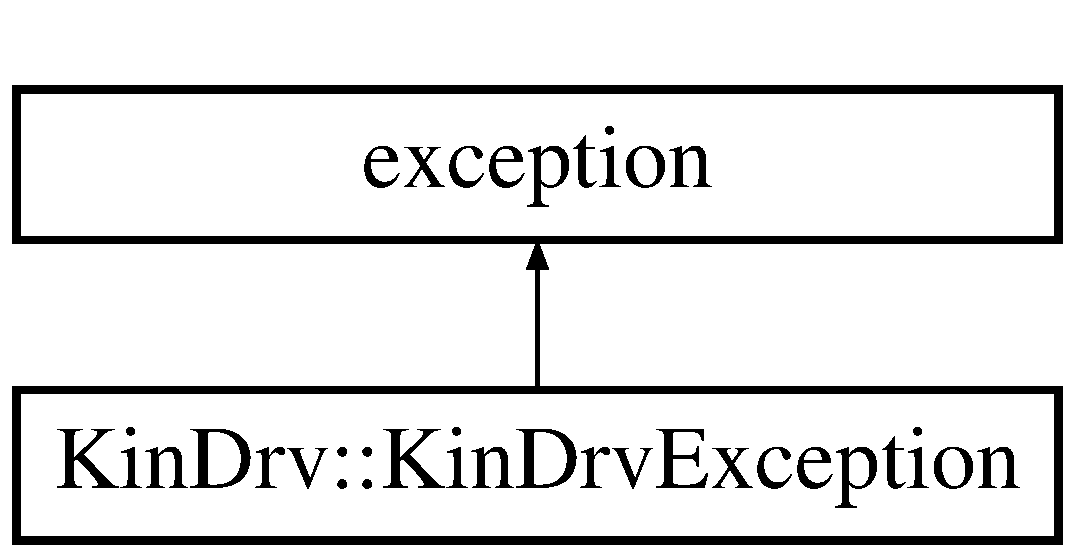
\includegraphics[height=2.000000cm]{classKinDrv_1_1KinDrvException}
\end{center}
\end{figure}
\subsection*{Public Member Functions}
\begin{DoxyCompactItemize}
\item 
\hyperlink{classKinDrv_1_1KinDrvException_a9de93afe0b9cb2789af4e1a90703c1ed}{Kin\+Drv\+Exception} ()  throw ()
\item 
\hyperlink{classKinDrv_1_1KinDrvException_aac037b5e448dad9cea4f30623514a853}{Kin\+Drv\+Exception} (const char $\ast$msg)  throw ()
\item 
\hyperlink{classKinDrv_1_1KinDrvException_ae4d643477d23b3f04119bc192fbaa42b}{Kin\+Drv\+Exception} (error\+\_\+t err, const char $\ast$msg)  throw ()
\item 
virtual \hyperlink{classKinDrv_1_1KinDrvException_aab87e6e6ddbf93de108d0fbd22543348}{$\sim$\+Kin\+Drv\+Exception} ()  throw ()
\item 
const char $\ast$ \hyperlink{classKinDrv_1_1KinDrvException_a7d1075b836e030e0c358821a8b26aaf0}{what} () const   throw ()
\item 
const error\+\_\+t \hyperlink{classKinDrv_1_1KinDrvException_af7f16d1830e8d54f5f373a743448011f}{error} () const   throw ()
\end{DoxyCompactItemize}


\subsection{Detailed Description}
Exception that is thrown by this Api. 

\subsection{Constructor \& Destructor Documentation}
\hypertarget{classKinDrv_1_1KinDrvException_a9de93afe0b9cb2789af4e1a90703c1ed}{\index{Kin\+Drv\+::\+Kin\+Drv\+Exception@{Kin\+Drv\+::\+Kin\+Drv\+Exception}!Kin\+Drv\+Exception@{Kin\+Drv\+Exception}}
\index{Kin\+Drv\+Exception@{Kin\+Drv\+Exception}!Kin\+Drv\+::\+Kin\+Drv\+Exception@{Kin\+Drv\+::\+Kin\+Drv\+Exception}}
\subsubsection[{Kin\+Drv\+Exception}]{\setlength{\rightskip}{0pt plus 5cm}Kin\+Drv\+::\+Kin\+Drv\+Exception\+::\+Kin\+Drv\+Exception (
\begin{DoxyParamCaption}
{}
\end{DoxyParamCaption}
) throw  ) }}\label{classKinDrv_1_1KinDrvException_a9de93afe0b9cb2789af4e1a90703c1ed}
Constructor. Constructs a new unknown exception with default parameters (type is E\+R\+R\+O\+R\+\_\+\+U\+N\+K\+N\+O\+W\+N, with \char`\"{}\+Unknown exception\char`\"{} as the message text). \hypertarget{classKinDrv_1_1KinDrvException_aac037b5e448dad9cea4f30623514a853}{\index{Kin\+Drv\+::\+Kin\+Drv\+Exception@{Kin\+Drv\+::\+Kin\+Drv\+Exception}!Kin\+Drv\+Exception@{Kin\+Drv\+Exception}}
\index{Kin\+Drv\+Exception@{Kin\+Drv\+Exception}!Kin\+Drv\+::\+Kin\+Drv\+Exception@{Kin\+Drv\+::\+Kin\+Drv\+Exception}}
\subsubsection[{Kin\+Drv\+Exception}]{\setlength{\rightskip}{0pt plus 5cm}Kin\+Drv\+::\+Kin\+Drv\+Exception\+::\+Kin\+Drv\+Exception (
\begin{DoxyParamCaption}
\item[{const char $\ast$}]{msg}
\end{DoxyParamCaption}
) throw  ) }}\label{classKinDrv_1_1KinDrvException_aac037b5e448dad9cea4f30623514a853}
Constructor. Constructs a new unknown exception (type is E\+R\+R\+O\+R\+\_\+\+U\+N\+K\+N\+O\+W\+N). The error message can be set manually. 
\begin{DoxyParams}{Parameters}
{\em msg} & The message text of the exception. \\
\hline
\end{DoxyParams}
\hypertarget{classKinDrv_1_1KinDrvException_ae4d643477d23b3f04119bc192fbaa42b}{\index{Kin\+Drv\+::\+Kin\+Drv\+Exception@{Kin\+Drv\+::\+Kin\+Drv\+Exception}!Kin\+Drv\+Exception@{Kin\+Drv\+Exception}}
\index{Kin\+Drv\+Exception@{Kin\+Drv\+Exception}!Kin\+Drv\+::\+Kin\+Drv\+Exception@{Kin\+Drv\+::\+Kin\+Drv\+Exception}}
\subsubsection[{Kin\+Drv\+Exception}]{\setlength{\rightskip}{0pt plus 5cm}Kin\+Drv\+::\+Kin\+Drv\+Exception\+::\+Kin\+Drv\+Exception (
\begin{DoxyParamCaption}
\item[{error\+\_\+t}]{err, }
\item[{const char $\ast$}]{msg}
\end{DoxyParamCaption}
) throw  ) }}\label{classKinDrv_1_1KinDrvException_ae4d643477d23b3f04119bc192fbaa42b}
Constructor. Constructs a new exception, type and message text can be set manually. 
\begin{DoxyParams}{Parameters}
{\em err} & The error type of this exception. \\
\hline
{\em msg} & The message text of the exception. \\
\hline
\end{DoxyParams}
\hypertarget{classKinDrv_1_1KinDrvException_aab87e6e6ddbf93de108d0fbd22543348}{\index{Kin\+Drv\+::\+Kin\+Drv\+Exception@{Kin\+Drv\+::\+Kin\+Drv\+Exception}!````~Kin\+Drv\+Exception@{$\sim$\+Kin\+Drv\+Exception}}
\index{````~Kin\+Drv\+Exception@{$\sim$\+Kin\+Drv\+Exception}!Kin\+Drv\+::\+Kin\+Drv\+Exception@{Kin\+Drv\+::\+Kin\+Drv\+Exception}}
\subsubsection[{$\sim$\+Kin\+Drv\+Exception}]{\setlength{\rightskip}{0pt plus 5cm}Kin\+Drv\+::\+Kin\+Drv\+Exception\+::$\sim$\+Kin\+Drv\+Exception (
\begin{DoxyParamCaption}
{}
\end{DoxyParamCaption}
) throw  ) \hspace{0.3cm}{\ttfamily [virtual]}}}\label{classKinDrv_1_1KinDrvException_aab87e6e6ddbf93de108d0fbd22543348}
Destructor. 

\subsection{Member Function Documentation}
\hypertarget{classKinDrv_1_1KinDrvException_af7f16d1830e8d54f5f373a743448011f}{\index{Kin\+Drv\+::\+Kin\+Drv\+Exception@{Kin\+Drv\+::\+Kin\+Drv\+Exception}!error@{error}}
\index{error@{error}!Kin\+Drv\+::\+Kin\+Drv\+Exception@{Kin\+Drv\+::\+Kin\+Drv\+Exception}}
\subsubsection[{error}]{\setlength{\rightskip}{0pt plus 5cm}const error\+\_\+t Kin\+Drv\+::\+Kin\+Drv\+Exception\+::error (
\begin{DoxyParamCaption}
{}
\end{DoxyParamCaption}
) const throw  ) }}\label{classKinDrv_1_1KinDrvException_af7f16d1830e8d54f5f373a743448011f}
Get the error type. \begin{DoxyReturn}{Returns}
The error type of the exception. 
\end{DoxyReturn}
\hypertarget{classKinDrv_1_1KinDrvException_a7d1075b836e030e0c358821a8b26aaf0}{\index{Kin\+Drv\+::\+Kin\+Drv\+Exception@{Kin\+Drv\+::\+Kin\+Drv\+Exception}!what@{what}}
\index{what@{what}!Kin\+Drv\+::\+Kin\+Drv\+Exception@{Kin\+Drv\+::\+Kin\+Drv\+Exception}}
\subsubsection[{what}]{\setlength{\rightskip}{0pt plus 5cm}const char $\ast$ Kin\+Drv\+::\+Kin\+Drv\+Exception\+::what (
\begin{DoxyParamCaption}
{}
\end{DoxyParamCaption}
) const throw  ) }}\label{classKinDrv_1_1KinDrvException_a7d1075b836e030e0c358821a8b26aaf0}
Get the error message. \begin{DoxyReturn}{Returns}
The error message of the exception. 
\end{DoxyReturn}


The documentation for this class was generated from the following files\+:\begin{DoxyCompactItemize}
\item 
exception.\+h\item 
exception.\+cpp\end{DoxyCompactItemize}

\hypertarget{classKinDrv_1_1mySerial}{\section{Kin\+Drv\+:\+:my\+Serial Class Reference}
\label{classKinDrv_1_1mySerial}\index{Kin\+Drv\+::my\+Serial@{Kin\+Drv\+::my\+Serial}}
}
\subsection*{Public Member Functions}
\begin{DoxyCompactItemize}
\item 
\hypertarget{classKinDrv_1_1mySerial_a2e1348a8a2ca2e6d3c54b1a9d4cac97e}{{\bfseries my\+Serial} (std\+::string device\+Name, int baud)}\label{classKinDrv_1_1mySerial_a2e1348a8a2ca2e6d3c54b1a9d4cac97e}

\item 
\hypertarget{classKinDrv_1_1mySerial_aaa0709c2a0da6caa74b51920651f41b0}{bool {\bfseries Send} (unsigned char $\ast$data, int len)}\label{classKinDrv_1_1mySerial_aaa0709c2a0da6caa74b51920651f41b0}

\item 
\hypertarget{classKinDrv_1_1mySerial_afda95bdbda913daae413f11e9c797d0b}{bool {\bfseries Send} (unsigned char value)}\label{classKinDrv_1_1mySerial_afda95bdbda913daae413f11e9c797d0b}

\item 
\hypertarget{classKinDrv_1_1mySerial_a8b5a2ddfef3eed88c01784bbb75b95fd}{bool {\bfseries Send} (std\+::string value)}\label{classKinDrv_1_1mySerial_a8b5a2ddfef3eed88c01784bbb75b95fd}

\item 
\hypertarget{classKinDrv_1_1mySerial_a2b31cda80376328f8ea3bc6b8b96f8f0}{int {\bfseries Receive} (unsigned char $\ast$data, int len)}\label{classKinDrv_1_1mySerial_a2b31cda80376328f8ea3bc6b8b96f8f0}

\item 
\hypertarget{classKinDrv_1_1mySerial_aa2586cbe30e33eb1a74d3f5d998c7a73}{bool {\bfseries Is\+Open} (void)}\label{classKinDrv_1_1mySerial_aa2586cbe30e33eb1a74d3f5d998c7a73}

\item 
\hypertarget{classKinDrv_1_1mySerial_a69d4a59899800a927334001449dda0b2}{void {\bfseries Close} (void)}\label{classKinDrv_1_1mySerial_a69d4a59899800a927334001449dda0b2}

\item 
\hypertarget{classKinDrv_1_1mySerial_a0e2518ebb88dd17a290c47684b210d00}{bool {\bfseries Open} (std\+::string device\+Name, int baud)}\label{classKinDrv_1_1mySerial_a0e2518ebb88dd17a290c47684b210d00}

\item 
\hypertarget{classKinDrv_1_1mySerial_aa57af296af4d11f53c51cf3e676a551e}{bool {\bfseries Number\+Byte\+Rcv} (int \&bytelen)}\label{classKinDrv_1_1mySerial_aa57af296af4d11f53c51cf3e676a551e}

\end{DoxyCompactItemize}
\subsection*{Public Attributes}
\begin{DoxyCompactItemize}
\item 
\hypertarget{classKinDrv_1_1mySerial_a92989cc09d53f00f5bf220608b216cb8}{int {\bfseries handle}}\label{classKinDrv_1_1mySerial_a92989cc09d53f00f5bf220608b216cb8}

\item 
\hypertarget{classKinDrv_1_1mySerial_a51c22dfc88cf528fdf17d2bceb7a11e9}{std\+::string {\bfseries device\+Name}}\label{classKinDrv_1_1mySerial_a51c22dfc88cf528fdf17d2bceb7a11e9}

\item 
\hypertarget{classKinDrv_1_1mySerial_a2ba702ee279deaa5f171747878417814}{int {\bfseries baud}}\label{classKinDrv_1_1mySerial_a2ba702ee279deaa5f171747878417814}

\end{DoxyCompactItemize}


The documentation for this class was generated from the following files\+:\begin{DoxyCompactItemize}
\item 
my\+Serial.\+h\item 
my\+Serial.\+cpp\end{DoxyCompactItemize}

\hypertarget{classKinDrv_1_1Robot__IMU__Control}{\section{Kin\+Drv\+:\+:Robot\+\_\+\+I\+M\+U\+\_\+\+Control Class Reference}
\label{classKinDrv_1_1Robot__IMU__Control}\index{Kin\+Drv\+::\+Robot\+\_\+\+I\+M\+U\+\_\+\+Control@{Kin\+Drv\+::\+Robot\+\_\+\+I\+M\+U\+\_\+\+Control}}
}
\subsection*{Public Member Functions}
\begin{DoxyCompactItemize}
\item 
\hypertarget{classKinDrv_1_1Robot__IMU__Control_a0e7b0fc8d61e08eedc29e5214218445a}{void {\bfseries read\+\_\+payload} (int data\mbox{[}$\,$\mbox{]})}\label{classKinDrv_1_1Robot__IMU__Control_a0e7b0fc8d61e08eedc29e5214218445a}

\item 
\hypertarget{classKinDrv_1_1Robot__IMU__Control_a6bc398065c2a7ae41057f8999dd3acb2}{void {\bfseries sensor\+\_\+fusion} ()}\label{classKinDrv_1_1Robot__IMU__Control_a6bc398065c2a7ae41057f8999dd3acb2}

\item 
\hypertarget{classKinDrv_1_1Robot__IMU__Control_a02498133fb9c8edfbd99ee44c6a36095}{void {\bfseries algo} ()}\label{classKinDrv_1_1Robot__IMU__Control_a02498133fb9c8edfbd99ee44c6a36095}

\item 
\hypertarget{classKinDrv_1_1Robot__IMU__Control_aceb015eb2e137c6b378397742bc3a057}{float {\bfseries C2\+\_\+2} (int var)}\label{classKinDrv_1_1Robot__IMU__Control_aceb015eb2e137c6b378397742bc3a057}

\item 
\hypertarget{classKinDrv_1_1Robot__IMU__Control_af6d18fb8a8a615e6fb6e1c9d1eea5389}{void {\bfseries wrap\+\_\+angle} (float $\ast$p\+\_\+angle)}\label{classKinDrv_1_1Robot__IMU__Control_af6d18fb8a8a615e6fb6e1c9d1eea5389}

\item 
\hypertarget{classKinDrv_1_1Robot__IMU__Control_a902e6312ccf4d73b8f11c6f77e00f411}{float {\bfseries rad2deg} (float angle\+\_\+rad)}\label{classKinDrv_1_1Robot__IMU__Control_a902e6312ccf4d73b8f11c6f77e00f411}

\item 
\hypertarget{classKinDrv_1_1Robot__IMU__Control_a11536918b5777f6829f044e227e0c469}{float {\bfseries deg2rad} (float angle\+\_\+deg)}\label{classKinDrv_1_1Robot__IMU__Control_a11536918b5777f6829f044e227e0c469}

\end{DoxyCompactItemize}
\subsection*{Public Attributes}
\begin{DoxyCompactItemize}
\item 
\hypertarget{classKinDrv_1_1Robot__IMU__Control_ab3a1152b8c5b61d4b8f36b78d356bd5f}{int {\bfseries F\+R\+E\+Q}}\label{classKinDrv_1_1Robot__IMU__Control_ab3a1152b8c5b61d4b8f36b78d356bd5f}

\item 
\hypertarget{classKinDrv_1_1Robot__IMU__Control_a67b09c5a182c499d389a286939346257}{int {\bfseries F\+R\+E\+Q\+\_\+\+B\+A\+S\+E}}\label{classKinDrv_1_1Robot__IMU__Control_a67b09c5a182c499d389a286939346257}

\item 
\hypertarget{classKinDrv_1_1Robot__IMU__Control_a09d2c358751309ad4c2899e1c0b6c7f7}{int {\bfseries sensor\+\_\+id}}\label{classKinDrv_1_1Robot__IMU__Control_a09d2c358751309ad4c2899e1c0b6c7f7}

\item 
\hypertarget{classKinDrv_1_1Robot__IMU__Control_aa69582e56667ce7d3a19a1e19b65f07d}{float {\bfseries Cmd\+X\+\_\+new}}\label{classKinDrv_1_1Robot__IMU__Control_aa69582e56667ce7d3a19a1e19b65f07d}

\item 
\hypertarget{classKinDrv_1_1Robot__IMU__Control_a0e717a559106527372d6eaf77194ff37}{float {\bfseries Cmd\+Y\+\_\+new}}\label{classKinDrv_1_1Robot__IMU__Control_a0e717a559106527372d6eaf77194ff37}

\item 
\hypertarget{classKinDrv_1_1Robot__IMU__Control_aabd37a633f049cfe54671d0bc5d0fe19}{float {\bfseries Cmd\+Xout}}\label{classKinDrv_1_1Robot__IMU__Control_aabd37a633f049cfe54671d0bc5d0fe19}

\item 
\hypertarget{classKinDrv_1_1Robot__IMU__Control_a4a6895a7433594063d4dcfaafa7c0fa5}{float {\bfseries Cmd\+Yout}}\label{classKinDrv_1_1Robot__IMU__Control_a4a6895a7433594063d4dcfaafa7c0fa5}

\item 
\hypertarget{classKinDrv_1_1Robot__IMU__Control_a9213ad8edccd586c052bd50108c44c96}{float {\bfseries Right\+Left\+Comm}}\label{classKinDrv_1_1Robot__IMU__Control_a9213ad8edccd586c052bd50108c44c96}

\item 
\hypertarget{classKinDrv_1_1Robot__IMU__Control_a7c9759c1fa4d10669d065df81da7b0a6}{float {\bfseries For\+Back\+Comm}}\label{classKinDrv_1_1Robot__IMU__Control_a7c9759c1fa4d10669d065df81da7b0a6}

\item 
\hypertarget{classKinDrv_1_1Robot__IMU__Control_ac31cdd510d009008fbcfff35d87ba294}{float {\bfseries Up\+Down\+Comm}}\label{classKinDrv_1_1Robot__IMU__Control_ac31cdd510d009008fbcfff35d87ba294}

\item 
\hypertarget{classKinDrv_1_1Robot__IMU__Control_a8f03d27c9446f3774ec9ee15c535c591}{float {\bfseries Right\+Left\+Comm\+\_\+ctrl}}\label{classKinDrv_1_1Robot__IMU__Control_a8f03d27c9446f3774ec9ee15c535c591}

\item 
\hypertarget{classKinDrv_1_1Robot__IMU__Control_aa78010d9a77b72f8295a6efb76723e68}{float {\bfseries For\+Back\+Comm\+\_\+ctrl}}\label{classKinDrv_1_1Robot__IMU__Control_aa78010d9a77b72f8295a6efb76723e68}

\item 
\hypertarget{classKinDrv_1_1Robot__IMU__Control_a92e817937103181a2987beba8a16e42f}{float {\bfseries Up\+Down\+Comm\+\_\+ctrl}}\label{classKinDrv_1_1Robot__IMU__Control_a92e817937103181a2987beba8a16e42f}

\item 
\hypertarget{classKinDrv_1_1Robot__IMU__Control_a5756ffeaaa494f2d951e627e675fbf1a}{float {\bfseries acc} \mbox{[}3\mbox{]}}\label{classKinDrv_1_1Robot__IMU__Control_a5756ffeaaa494f2d951e627e675fbf1a}

\item 
\hypertarget{classKinDrv_1_1Robot__IMU__Control_ac80be63e8705bda7b4b05bec11cac607}{float {\bfseries gyr} \mbox{[}3\mbox{]}}\label{classKinDrv_1_1Robot__IMU__Control_ac80be63e8705bda7b4b05bec11cac607}

\item 
\hypertarget{classKinDrv_1_1Robot__IMU__Control_a47715b005dc25bf1c60fb5b276b35672}{float {\bfseries mag} \mbox{[}3\mbox{]}}\label{classKinDrv_1_1Robot__IMU__Control_a47715b005dc25bf1c60fb5b276b35672}

\item 
\hypertarget{classKinDrv_1_1Robot__IMU__Control_ad018afd043c36d4b9d00ef08b52a590b}{float {\bfseries pitch} \mbox{[}3\mbox{]}}\label{classKinDrv_1_1Robot__IMU__Control_ad018afd043c36d4b9d00ef08b52a590b}

\item 
\hypertarget{classKinDrv_1_1Robot__IMU__Control_a3c1f3da002eb6052753c158bfe4c6171}{float {\bfseries x\+\_\+pitch} \mbox{[}3\mbox{]}}\label{classKinDrv_1_1Robot__IMU__Control_a3c1f3da002eb6052753c158bfe4c6171}

\item 
\hypertarget{classKinDrv_1_1Robot__IMU__Control_a30910897a585aba2b7eaec4fc90ebcfd}{float {\bfseries roll} \mbox{[}3\mbox{]}}\label{classKinDrv_1_1Robot__IMU__Control_a30910897a585aba2b7eaec4fc90ebcfd}

\item 
\hypertarget{classKinDrv_1_1Robot__IMU__Control_a94b2d82c7d0b8b3e7751a8d578db53a8}{float {\bfseries x\+\_\+roll} \mbox{[}3\mbox{]}}\label{classKinDrv_1_1Robot__IMU__Control_a94b2d82c7d0b8b3e7751a8d578db53a8}

\item 
\hypertarget{classKinDrv_1_1Robot__IMU__Control_a8d2ee7b27c87d4191073cefdce949fd2}{float {\bfseries yaw} \mbox{[}3\mbox{]}}\label{classKinDrv_1_1Robot__IMU__Control_a8d2ee7b27c87d4191073cefdce949fd2}

\item 
\hypertarget{classKinDrv_1_1Robot__IMU__Control_acb350e47745d0c70476855481a4fff3c}{float {\bfseries x\+\_\+yaw} \mbox{[}3\mbox{]}}\label{classKinDrv_1_1Robot__IMU__Control_acb350e47745d0c70476855481a4fff3c}

\item 
\hypertarget{classKinDrv_1_1Robot__IMU__Control_ab264a1cb9d29dc487dc000073377b80e}{float {\bfseries x}}\label{classKinDrv_1_1Robot__IMU__Control_ab264a1cb9d29dc487dc000073377b80e}

\item 
\hypertarget{classKinDrv_1_1Robot__IMU__Control_a07ff0f1d9c98ed12e32d3c69415aa950}{float {\bfseries y}}\label{classKinDrv_1_1Robot__IMU__Control_a07ff0f1d9c98ed12e32d3c69415aa950}

\item 
\hypertarget{classKinDrv_1_1Robot__IMU__Control_a8d065c697fe41c89a1b80f3547017cce}{float {\bfseries x0}}\label{classKinDrv_1_1Robot__IMU__Control_a8d065c697fe41c89a1b80f3547017cce}

\item 
\hypertarget{classKinDrv_1_1Robot__IMU__Control_a5810e687fe7ba00098a9354652a1dfee}{float {\bfseries y0}}\label{classKinDrv_1_1Robot__IMU__Control_a5810e687fe7ba00098a9354652a1dfee}

\item 
\hypertarget{classKinDrv_1_1Robot__IMU__Control_a23bd6fe9de197940095281cda6735daa}{float {\bfseries xoff}}\label{classKinDrv_1_1Robot__IMU__Control_a23bd6fe9de197940095281cda6735daa}

\item 
\hypertarget{classKinDrv_1_1Robot__IMU__Control_a885225f3d14e5c59c190becbe938b65a}{float {\bfseries yoff}}\label{classKinDrv_1_1Robot__IMU__Control_a885225f3d14e5c59c190becbe938b65a}

\item 
\hypertarget{classKinDrv_1_1Robot__IMU__Control_a46dcedc90f78635d3a036857b5259a1c}{float {\bfseries Amp}}\label{classKinDrv_1_1Robot__IMU__Control_a46dcedc90f78635d3a036857b5259a1c}

\item 
\hypertarget{classKinDrv_1_1Robot__IMU__Control_a14b0c11bd47f2dda913c40e69cbc8014}{float {\bfseries Theta}}\label{classKinDrv_1_1Robot__IMU__Control_a14b0c11bd47f2dda913c40e69cbc8014}

\item 
\hypertarget{classKinDrv_1_1Robot__IMU__Control_a6d838dc9153a74bdb2014b5a9b2f5491}{float {\bfseries Orientation}}\label{classKinDrv_1_1Robot__IMU__Control_a6d838dc9153a74bdb2014b5a9b2f5491}

\item 
\hypertarget{classKinDrv_1_1Robot__IMU__Control_a905ee91787396fe7e0d72cb334ae7430}{int {\bfseries Valid}}\label{classKinDrv_1_1Robot__IMU__Control_a905ee91787396fe7e0d72cb334ae7430}

\item 
\hypertarget{classKinDrv_1_1Robot__IMU__Control_ac63372a655258fe90d637212dcbaa44a}{int {\bfseries Diago\+Active}}\label{classKinDrv_1_1Robot__IMU__Control_ac63372a655258fe90d637212dcbaa44a}

\item 
\hypertarget{classKinDrv_1_1Robot__IMU__Control_af858b8ea6c7aa1c831422aa5bf5e59d7}{float {\bfseries Theta\+\_\+offset}}\label{classKinDrv_1_1Robot__IMU__Control_af858b8ea6c7aa1c831422aa5bf5e59d7}

\item 
\hypertarget{classKinDrv_1_1Robot__IMU__Control_a9819b5ebe27cc799607c525a3cb4634c}{float {\bfseries Amin\+\_\+\+B\+A\+C\+K}}\label{classKinDrv_1_1Robot__IMU__Control_a9819b5ebe27cc799607c525a3cb4634c}

\item 
\hypertarget{classKinDrv_1_1Robot__IMU__Control_aeb32167cf9ae623f9ab10a869159de34}{float {\bfseries Amax\+\_\+\+B\+A\+C\+K}}\label{classKinDrv_1_1Robot__IMU__Control_aeb32167cf9ae623f9ab10a869159de34}

\item 
\hypertarget{classKinDrv_1_1Robot__IMU__Control_a789fe5f2ec5da388c1f6d16589e2590d}{float {\bfseries Amin\+\_\+\+D}}\label{classKinDrv_1_1Robot__IMU__Control_a789fe5f2ec5da388c1f6d16589e2590d}

\item 
\hypertarget{classKinDrv_1_1Robot__IMU__Control_a19a3de909040904686b0c7eae7029c75}{float {\bfseries Amax\+\_\+\+D}}\label{classKinDrv_1_1Robot__IMU__Control_a19a3de909040904686b0c7eae7029c75}

\item 
\hypertarget{classKinDrv_1_1Robot__IMU__Control_aa1ec8896a1bf8ac2382df3ea7af0d746}{float {\bfseries Amax}}\label{classKinDrv_1_1Robot__IMU__Control_aa1ec8896a1bf8ac2382df3ea7af0d746}

\item 
\hypertarget{classKinDrv_1_1Robot__IMU__Control_ae01094ba1a278304e9e3b4201e4d0409}{float {\bfseries Amin}}\label{classKinDrv_1_1Robot__IMU__Control_ae01094ba1a278304e9e3b4201e4d0409}

\item 
\hypertarget{classKinDrv_1_1Robot__IMU__Control_a2043e2c551e716a61a85d7f282f84544}{float {\bfseries Zone\+Forw}}\label{classKinDrv_1_1Robot__IMU__Control_a2043e2c551e716a61a85d7f282f84544}

\item 
\hypertarget{classKinDrv_1_1Robot__IMU__Control_a913681ea8551679b49a369aae1325532}{float {\bfseries Delta\+Forw}}\label{classKinDrv_1_1Robot__IMU__Control_a913681ea8551679b49a369aae1325532}

\item 
\hypertarget{classKinDrv_1_1Robot__IMU__Control_abd17acf8f3f2b8d3ddc237ac235748ce}{float {\bfseries Zone\+Right}}\label{classKinDrv_1_1Robot__IMU__Control_abd17acf8f3f2b8d3ddc237ac235748ce}

\item 
\hypertarget{classKinDrv_1_1Robot__IMU__Control_af9e6c9fb4f23a5a90cc3b70bc67be606}{float {\bfseries Delta\+Right}}\label{classKinDrv_1_1Robot__IMU__Control_af9e6c9fb4f23a5a90cc3b70bc67be606}

\item 
\hypertarget{classKinDrv_1_1Robot__IMU__Control_a0d93ed805a0cce1246dc8dbfc8cfb2f4}{float {\bfseries Zone\+Left}}\label{classKinDrv_1_1Robot__IMU__Control_a0d93ed805a0cce1246dc8dbfc8cfb2f4}

\item 
\hypertarget{classKinDrv_1_1Robot__IMU__Control_a792a59594362605aacdc26db26b3000a}{float {\bfseries Delta\+Left}}\label{classKinDrv_1_1Robot__IMU__Control_a792a59594362605aacdc26db26b3000a}

\item 
\hypertarget{classKinDrv_1_1Robot__IMU__Control_ad04b3ca655793f693c7f504bc4e98132}{float {\bfseries Zone\+Back}}\label{classKinDrv_1_1Robot__IMU__Control_ad04b3ca655793f693c7f504bc4e98132}

\item 
\hypertarget{classKinDrv_1_1Robot__IMU__Control_a7358960d6a32d4de5daddfed7fa53109}{float {\bfseries Delta\+Back}}\label{classKinDrv_1_1Robot__IMU__Control_a7358960d6a32d4de5daddfed7fa53109}

\item 
\hypertarget{classKinDrv_1_1Robot__IMU__Control_a4194ac6289efe9cd9bdddad32fa0b406}{float {\bfseries Max\+Up}}\label{classKinDrv_1_1Robot__IMU__Control_a4194ac6289efe9cd9bdddad32fa0b406}

\item 
\hypertarget{classKinDrv_1_1Robot__IMU__Control_abae05a420b11096c7fed3445cf326ab5}{float {\bfseries Delta\+Max\+Up}}\label{classKinDrv_1_1Robot__IMU__Control_abae05a420b11096c7fed3445cf326ab5}

\item 
\hypertarget{classKinDrv_1_1Robot__IMU__Control_abd1e59546d5e3a2602e90c3ca0a02cf8}{float {\bfseries Max\+Down}}\label{classKinDrv_1_1Robot__IMU__Control_abd1e59546d5e3a2602e90c3ca0a02cf8}

\item 
\hypertarget{classKinDrv_1_1Robot__IMU__Control_ab22873a1bdc221ef234e2672c58ce922}{float {\bfseries Delta\+Max\+Down}}\label{classKinDrv_1_1Robot__IMU__Control_ab22873a1bdc221ef234e2672c58ce922}

\item 
\hypertarget{classKinDrv_1_1Robot__IMU__Control_a1c4939489fb0b4a2c08feea19b867f30}{float {\bfseries Neutral\+Up\+Down}}\label{classKinDrv_1_1Robot__IMU__Control_a1c4939489fb0b4a2c08feea19b867f30}

\item 
\hypertarget{classKinDrv_1_1Robot__IMU__Control_a7fc73a918cd3283c802614cee87ada6e}{float {\bfseries Delta\+Neutral\+Up\+Down}}\label{classKinDrv_1_1Robot__IMU__Control_a7fc73a918cd3283c802614cee87ada6e}

\item 
\hypertarget{classKinDrv_1_1Robot__IMU__Control_a511004d28f76e0eedf1ba2413ac506e8}{int {\bfseries P\+R\+E\+S\+S\+E\+D}}\label{classKinDrv_1_1Robot__IMU__Control_a511004d28f76e0eedf1ba2413ac506e8}

\item 
\hypertarget{classKinDrv_1_1Robot__IMU__Control_aca468d5095699476f962f94939ca2db4}{int {\bfseries pressedtime}}\label{classKinDrv_1_1Robot__IMU__Control_aca468d5095699476f962f94939ca2db4}

\item 
\hypertarget{classKinDrv_1_1Robot__IMU__Control_a2fb4e0deba27858fb6b02d7e84906738}{int {\bfseries B\+\_\+\+I\+N\+D\+E\+X}}\label{classKinDrv_1_1Robot__IMU__Control_a2fb4e0deba27858fb6b02d7e84906738}

\item 
\hypertarget{classKinDrv_1_1Robot__IMU__Control_aa76b23776476baaac33f2fd8f9555d91}{bool {\bfseries H\+O\+M\+E\+\_\+\+P\+R\+E\+S\+S\+E\+D}}\label{classKinDrv_1_1Robot__IMU__Control_aa76b23776476baaac33f2fd8f9555d91}

\item 
\hypertarget{classKinDrv_1_1Robot__IMU__Control_a6cd41dfcee9221d6171ea545eeb96cb7}{bool {\bfseries B\+A\+C\+K}}\label{classKinDrv_1_1Robot__IMU__Control_a6cd41dfcee9221d6171ea545eeb96cb7}

\end{DoxyCompactItemize}
\subsection*{Static Public Attributes}
\begin{DoxyCompactItemize}
\item 
\hypertarget{classKinDrv_1_1Robot__IMU__Control_aa2fc25bf279cb217eb7922349ed7342c}{static const double {\bfseries num\+\_\+lp\+\_\+10\+Hz} \mbox{[}3\mbox{]} = \{ 0.\+355, 0.\+355, 0.\+0 \}}\label{classKinDrv_1_1Robot__IMU__Control_aa2fc25bf279cb217eb7922349ed7342c}

\item 
\hypertarget{classKinDrv_1_1Robot__IMU__Control_a73d77428f98c333ba1c28854ff842aae}{static const double {\bfseries num\+\_\+lp\+\_\+25\+Hz} \mbox{[}3\mbox{]} = \{ 0.\+755, 0.\+755, 0.\+0 \}}\label{classKinDrv_1_1Robot__IMU__Control_a73d77428f98c333ba1c28854ff842aae}

\item 
\hypertarget{classKinDrv_1_1Robot__IMU__Control_ae0cf744e68ddfc1ecd54386cae50ac68}{static const double {\bfseries den\+\_\+lp\+\_\+10\+Hz} \mbox{[}3\mbox{]} = \{ 1.\+0, -\/0.\+2905, 0.\+0 \}}\label{classKinDrv_1_1Robot__IMU__Control_ae0cf744e68ddfc1ecd54386cae50ac68}

\item 
\hypertarget{classKinDrv_1_1Robot__IMU__Control_ae24f49173560ac964ffd9749e22e90f9}{static const double {\bfseries den\+\_\+lp\+\_\+25\+Hz} \mbox{[}3\mbox{]} = \{ 1.\+0, 0.\+5095, 0.\+0 \}}\label{classKinDrv_1_1Robot__IMU__Control_ae24f49173560ac964ffd9749e22e90f9}

\item 
static const double {\bfseries comp\+\_\+headset} \mbox{[}3\mbox{]}\mbox{[}3\mbox{]}
\item 
\hypertarget{classKinDrv_1_1Robot__IMU__Control_a6f50736a1e8c2ad27e08bdc890ebb5bb}{static const double {\bfseries hardiron\+\_\+headset} \mbox{[}3\mbox{]} = \{ -\/725.\+100317519760, 491.\+703440889862, -\/53.\+3108814506022 \}}\label{classKinDrv_1_1Robot__IMU__Control_a6f50736a1e8c2ad27e08bdc890ebb5bb}

\end{DoxyCompactItemize}


\subsection{Member Data Documentation}
\hypertarget{classKinDrv_1_1Robot__IMU__Control_a1acf749d1d1d97813baeecf0c8b74830}{\index{Kin\+Drv\+::\+Robot\+\_\+\+I\+M\+U\+\_\+\+Control@{Kin\+Drv\+::\+Robot\+\_\+\+I\+M\+U\+\_\+\+Control}!comp\+\_\+headset@{comp\+\_\+headset}}
\index{comp\+\_\+headset@{comp\+\_\+headset}!Kin\+Drv\+::\+Robot\+\_\+\+I\+M\+U\+\_\+\+Control@{Kin\+Drv\+::\+Robot\+\_\+\+I\+M\+U\+\_\+\+Control}}
\subsubsection[{comp\+\_\+headset}]{\setlength{\rightskip}{0pt plus 5cm}const double Kin\+Drv\+::\+Robot\+\_\+\+I\+M\+U\+\_\+\+Control\+::comp\+\_\+headset\hspace{0.3cm}{\ttfamily [static]}}}\label{classKinDrv_1_1Robot__IMU__Control_a1acf749d1d1d97813baeecf0c8b74830}
{\bfseries Initial value\+:}
\begin{DoxyCode}
= \{ \{ 0.000168679716274983, -5.17710741425967e-06, -8.77884394210979e-07 \},
                                                                                                           
      \{ -5.17710741425967e-06, 0.000159571222440490, -3.27611632378113e-06 \},
                                                                                                           
      \{ -8.77884394210986e-07, -3.27611632378113e-06, 0.000166456977421752 \} \}
\end{DoxyCode}


The documentation for this class was generated from the following files\+:\begin{DoxyCompactItemize}
\item 
Robot\+\_\+\+I\+M\+U\+\_\+\+Control.\+h\item 
Robot\+\_\+\+I\+M\+U\+\_\+\+Control.\+cpp\end{DoxyCompactItemize}

\hypertarget{structKinDrv_1_1usb__device__struct}{\section{Kin\+Drv\+:\+:usb\+\_\+device\+\_\+struct Struct Reference}
\label{structKinDrv_1_1usb__device__struct}\index{Kin\+Drv\+::usb\+\_\+device\+\_\+struct@{Kin\+Drv\+::usb\+\_\+device\+\_\+struct}}
}
\subsection*{Public Attributes}
\begin{DoxyCompactItemize}
\item 
unsigned int \hyperlink{structKinDrv_1_1usb__device__struct_a0e6de35dc6c03706c83ace64c9febb37}{bus}
\item 
unsigned int \hyperlink{structKinDrv_1_1usb__device__struct_a68e7077ad8819f255088238f9b1cd252}{address}
\item 
libusb\+\_\+device $\ast$ \hyperlink{structKinDrv_1_1usb__device__struct_a9b0ea0b72fe367e18da99404e9d57c9d}{dev}
\item 
bool \hyperlink{structKinDrv_1_1usb__device__struct_a5edef24a9b1076404c9ab42410c82952}{connected}
\item 
char \hyperlink{structKinDrv_1_1usb__device__struct_a03a9e83a8e46ac647654302ceafb2a5f}{client\+\_\+name} \mbox{[}20\mbox{]}
\end{DoxyCompactItemize}


\subsection{Detailed Description}
struct for internal usage only! stores U\+S\+B info about connected arms 

\subsection{Member Data Documentation}
\hypertarget{structKinDrv_1_1usb__device__struct_a68e7077ad8819f255088238f9b1cd252}{\index{Kin\+Drv\+::usb\+\_\+device\+\_\+struct@{Kin\+Drv\+::usb\+\_\+device\+\_\+struct}!address@{address}}
\index{address@{address}!Kin\+Drv\+::usb\+\_\+device\+\_\+struct@{Kin\+Drv\+::usb\+\_\+device\+\_\+struct}}
\subsubsection[{address}]{\setlength{\rightskip}{0pt plus 5cm}unsigned int Kin\+Drv\+::usb\+\_\+device\+\_\+struct\+::address}}\label{structKinDrv_1_1usb__device__struct_a68e7077ad8819f255088238f9b1cd252}
U\+S\+B device address \hypertarget{structKinDrv_1_1usb__device__struct_a0e6de35dc6c03706c83ace64c9febb37}{\index{Kin\+Drv\+::usb\+\_\+device\+\_\+struct@{Kin\+Drv\+::usb\+\_\+device\+\_\+struct}!bus@{bus}}
\index{bus@{bus}!Kin\+Drv\+::usb\+\_\+device\+\_\+struct@{Kin\+Drv\+::usb\+\_\+device\+\_\+struct}}
\subsubsection[{bus}]{\setlength{\rightskip}{0pt plus 5cm}unsigned int Kin\+Drv\+::usb\+\_\+device\+\_\+struct\+::bus}}\label{structKinDrv_1_1usb__device__struct_a0e6de35dc6c03706c83ace64c9febb37}
U\+S\+B bus number \hypertarget{structKinDrv_1_1usb__device__struct_a03a9e83a8e46ac647654302ceafb2a5f}{\index{Kin\+Drv\+::usb\+\_\+device\+\_\+struct@{Kin\+Drv\+::usb\+\_\+device\+\_\+struct}!client\+\_\+name@{client\+\_\+name}}
\index{client\+\_\+name@{client\+\_\+name}!Kin\+Drv\+::usb\+\_\+device\+\_\+struct@{Kin\+Drv\+::usb\+\_\+device\+\_\+struct}}
\subsubsection[{client\+\_\+name}]{\setlength{\rightskip}{0pt plus 5cm}char Kin\+Drv\+::usb\+\_\+device\+\_\+struct\+::client\+\_\+name\mbox{[}20\mbox{]}}}\label{structKinDrv_1_1usb__device__struct_a03a9e83a8e46ac647654302ceafb2a5f}
The name of the Arm (from client\+\_\+config) \hypertarget{structKinDrv_1_1usb__device__struct_a5edef24a9b1076404c9ab42410c82952}{\index{Kin\+Drv\+::usb\+\_\+device\+\_\+struct@{Kin\+Drv\+::usb\+\_\+device\+\_\+struct}!connected@{connected}}
\index{connected@{connected}!Kin\+Drv\+::usb\+\_\+device\+\_\+struct@{Kin\+Drv\+::usb\+\_\+device\+\_\+struct}}
\subsubsection[{connected}]{\setlength{\rightskip}{0pt plus 5cm}bool Kin\+Drv\+::usb\+\_\+device\+\_\+struct\+::connected}}\label{structKinDrv_1_1usb__device__struct_a5edef24a9b1076404c9ab42410c82952}
Indicates if arm is in use (connected; has a device\+\_\+handler) or not \hypertarget{structKinDrv_1_1usb__device__struct_a9b0ea0b72fe367e18da99404e9d57c9d}{\index{Kin\+Drv\+::usb\+\_\+device\+\_\+struct@{Kin\+Drv\+::usb\+\_\+device\+\_\+struct}!dev@{dev}}
\index{dev@{dev}!Kin\+Drv\+::usb\+\_\+device\+\_\+struct@{Kin\+Drv\+::usb\+\_\+device\+\_\+struct}}
\subsubsection[{dev}]{\setlength{\rightskip}{0pt plus 5cm}libusb\+\_\+device$\ast$ Kin\+Drv\+::usb\+\_\+device\+\_\+struct\+::dev}}\label{structKinDrv_1_1usb__device__struct_a9b0ea0b72fe367e18da99404e9d57c9d}
libusb\+\_\+device pointer; refed 

The documentation for this struct was generated from the following file\+:\begin{DoxyCompactItemize}
\item 
kindrv.\+cpp\end{DoxyCompactItemize}

\hypertarget{structKinDrv_1_1usb__packet__header__t}{\section{Kin\+Drv\+:\+:usb\+\_\+packet\+\_\+header\+\_\+t Struct Reference}
\label{structKinDrv_1_1usb__packet__header__t}\index{Kin\+Drv\+::usb\+\_\+packet\+\_\+header\+\_\+t@{Kin\+Drv\+::usb\+\_\+packet\+\_\+header\+\_\+t}}
}


U\+S\+B packet header struct. All U\+S\+B packets must have this header structure.  




{\ttfamily \#include $<$types.\+h$>$}

\subsection*{Public Attributes}
\begin{DoxyCompactItemize}
\item 
unsigned short \hyperlink{structKinDrv_1_1usb__packet__header__t_a960ee443a2288035f5a8dde73156b09a}{id\+\_\+packet}
\item 
unsigned short \hyperlink{structKinDrv_1_1usb__packet__header__t_a1e7318460cae97671f9f2b2488c25e58}{packet\+\_\+quantity}
\item 
unsigned short \hyperlink{structKinDrv_1_1usb__packet__header__t_a7efa30260f38c095ba9d3496fc1f6ca3}{command\+\_\+id}
\item 
unsigned short \hyperlink{structKinDrv_1_1usb__packet__header__t_a1c5726c153fb8c111224abad09f89769}{command\+\_\+size}
\end{DoxyCompactItemize}


\subsection{Detailed Description}
U\+S\+B packet header struct. All U\+S\+B packets must have this header structure. 

\subsection{Member Data Documentation}
\hypertarget{structKinDrv_1_1usb__packet__header__t_a7efa30260f38c095ba9d3496fc1f6ca3}{\index{Kin\+Drv\+::usb\+\_\+packet\+\_\+header\+\_\+t@{Kin\+Drv\+::usb\+\_\+packet\+\_\+header\+\_\+t}!command\+\_\+id@{command\+\_\+id}}
\index{command\+\_\+id@{command\+\_\+id}!Kin\+Drv\+::usb\+\_\+packet\+\_\+header\+\_\+t@{Kin\+Drv\+::usb\+\_\+packet\+\_\+header\+\_\+t}}
\subsubsection[{command\+\_\+id}]{\setlength{\rightskip}{0pt plus 5cm}unsigned short Kin\+Drv\+::usb\+\_\+packet\+\_\+header\+\_\+t\+::command\+\_\+id}}\label{structKinDrv_1_1usb__packet__header__t_a7efa30260f38c095ba9d3496fc1f6ca3}
The command id. \hypertarget{structKinDrv_1_1usb__packet__header__t_a1c5726c153fb8c111224abad09f89769}{\index{Kin\+Drv\+::usb\+\_\+packet\+\_\+header\+\_\+t@{Kin\+Drv\+::usb\+\_\+packet\+\_\+header\+\_\+t}!command\+\_\+size@{command\+\_\+size}}
\index{command\+\_\+size@{command\+\_\+size}!Kin\+Drv\+::usb\+\_\+packet\+\_\+header\+\_\+t@{Kin\+Drv\+::usb\+\_\+packet\+\_\+header\+\_\+t}}
\subsubsection[{command\+\_\+size}]{\setlength{\rightskip}{0pt plus 5cm}unsigned short Kin\+Drv\+::usb\+\_\+packet\+\_\+header\+\_\+t\+::command\+\_\+size}}\label{structKinDrv_1_1usb__packet__header__t_a1c5726c153fb8c111224abad09f89769}
The total size of the command data (in bytes) that is transmitted. \hypertarget{structKinDrv_1_1usb__packet__header__t_a960ee443a2288035f5a8dde73156b09a}{\index{Kin\+Drv\+::usb\+\_\+packet\+\_\+header\+\_\+t@{Kin\+Drv\+::usb\+\_\+packet\+\_\+header\+\_\+t}!id\+\_\+packet@{id\+\_\+packet}}
\index{id\+\_\+packet@{id\+\_\+packet}!Kin\+Drv\+::usb\+\_\+packet\+\_\+header\+\_\+t@{Kin\+Drv\+::usb\+\_\+packet\+\_\+header\+\_\+t}}
\subsubsection[{id\+\_\+packet}]{\setlength{\rightskip}{0pt plus 5cm}unsigned short Kin\+Drv\+::usb\+\_\+packet\+\_\+header\+\_\+t\+::id\+\_\+packet}}\label{structKinDrv_1_1usb__packet__header__t_a960ee443a2288035f5a8dde73156b09a}
The packet id. \hypertarget{structKinDrv_1_1usb__packet__header__t_a1e7318460cae97671f9f2b2488c25e58}{\index{Kin\+Drv\+::usb\+\_\+packet\+\_\+header\+\_\+t@{Kin\+Drv\+::usb\+\_\+packet\+\_\+header\+\_\+t}!packet\+\_\+quantity@{packet\+\_\+quantity}}
\index{packet\+\_\+quantity@{packet\+\_\+quantity}!Kin\+Drv\+::usb\+\_\+packet\+\_\+header\+\_\+t@{Kin\+Drv\+::usb\+\_\+packet\+\_\+header\+\_\+t}}
\subsubsection[{packet\+\_\+quantity}]{\setlength{\rightskip}{0pt plus 5cm}unsigned short Kin\+Drv\+::usb\+\_\+packet\+\_\+header\+\_\+t\+::packet\+\_\+quantity}}\label{structKinDrv_1_1usb__packet__header__t_a1e7318460cae97671f9f2b2488c25e58}
Total number of packets, that are transmitted for this command. 

The documentation for this struct was generated from the following file\+:\begin{DoxyCompactItemize}
\item 
types.\+h\end{DoxyCompactItemize}

\hypertarget{structKinDrv_1_1usb__packet__t}{\section{Kin\+Drv\+:\+:usb\+\_\+packet\+\_\+t Struct Reference}
\label{structKinDrv_1_1usb__packet__t}\index{Kin\+Drv\+::usb\+\_\+packet\+\_\+t@{Kin\+Drv\+::usb\+\_\+packet\+\_\+t}}
}


U\+S\+B packet struct. All U\+S\+B I/\+O is one of this.  




{\ttfamily \#include $<$types.\+h$>$}

\subsection*{Public Attributes}
\begin{DoxyCompactItemize}
\item 
\hypertarget{structKinDrv_1_1usb__packet__t_aaa785bbcefa917391ae5a335316b26d0}{\begin{tabbing}
xx\=xx\=xx\=xx\=xx\=xx\=xx\=xx\=xx\=\kill
union \{\\
\>unsigned char \hyperlink{structKinDrv_1_1usb__packet__t_a1c148e5f7d4aa73edf4dd14446599392}{data} \mbox{[}64\mbox{]}\\
\hypertarget{unionKinDrv_1_1usb__packet__t_1_1@12_a7f8ba3677f5ce5341429feec63b5bece}{\>struct \{\\
\>\>\hyperlink{structKinDrv_1_1usb__packet__header__t}{usb\_packet\_header\_t} \hyperlink{structKinDrv_1_1usb__packet__t_a78c5d7c50d214e862212893920c112d7}{header}\\
\>\>float \hyperlink{structKinDrv_1_1usb__packet__t_aaf50aa504bd699a24581d8a53dbaa52c}{body} \mbox{[}14\mbox{]}\\
\>\} }\label{unionKinDrv_1_1usb__packet__t_1_1@12_a7f8ba3677f5ce5341429feec63b5bece}
\\
\}; }\label{structKinDrv_1_1usb__packet__t_aaa785bbcefa917391ae5a335316b26d0}
\\

\end{tabbing}\end{DoxyCompactItemize}


\subsection{Detailed Description}
U\+S\+B packet struct. All U\+S\+B I/\+O is one of this. 

\subsection{Member Data Documentation}
\hypertarget{structKinDrv_1_1usb__packet__t_aaf50aa504bd699a24581d8a53dbaa52c}{\index{Kin\+Drv\+::usb\+\_\+packet\+\_\+t@{Kin\+Drv\+::usb\+\_\+packet\+\_\+t}!body@{body}}
\index{body@{body}!Kin\+Drv\+::usb\+\_\+packet\+\_\+t@{Kin\+Drv\+::usb\+\_\+packet\+\_\+t}}
\subsubsection[{body}]{\setlength{\rightskip}{0pt plus 5cm}float Kin\+Drv\+::usb\+\_\+packet\+\_\+t\+::body\mbox{[}14\mbox{]}}}\label{structKinDrv_1_1usb__packet__t_aaf50aa504bd699a24581d8a53dbaa52c}
56 byte body, containing the actual data. \hypertarget{structKinDrv_1_1usb__packet__t_a1c148e5f7d4aa73edf4dd14446599392}{\index{Kin\+Drv\+::usb\+\_\+packet\+\_\+t@{Kin\+Drv\+::usb\+\_\+packet\+\_\+t}!data@{data}}
\index{data@{data}!Kin\+Drv\+::usb\+\_\+packet\+\_\+t@{Kin\+Drv\+::usb\+\_\+packet\+\_\+t}}
\subsubsection[{data}]{\setlength{\rightskip}{0pt plus 5cm}unsigned char Kin\+Drv\+::usb\+\_\+packet\+\_\+t\+::data\mbox{[}64\mbox{]}}}\label{structKinDrv_1_1usb__packet__t_a1c148e5f7d4aa73edf4dd14446599392}
Access the whole 64 bytes of raw data. \hypertarget{structKinDrv_1_1usb__packet__t_a78c5d7c50d214e862212893920c112d7}{\index{Kin\+Drv\+::usb\+\_\+packet\+\_\+t@{Kin\+Drv\+::usb\+\_\+packet\+\_\+t}!header@{header}}
\index{header@{header}!Kin\+Drv\+::usb\+\_\+packet\+\_\+t@{Kin\+Drv\+::usb\+\_\+packet\+\_\+t}}
\subsubsection[{header}]{\setlength{\rightskip}{0pt plus 5cm}{\bf usb\+\_\+packet\+\_\+header\+\_\+t} Kin\+Drv\+::usb\+\_\+packet\+\_\+t\+::header}}\label{structKinDrv_1_1usb__packet__t_a78c5d7c50d214e862212893920c112d7}
8 byte header information. 

The documentation for this struct was generated from the following file\+:\begin{DoxyCompactItemize}
\item 
types.\+h\end{DoxyCompactItemize}

%--- End generated contents ---

% Index
\newpage
\phantomsection
\addcontentsline{toc}{chapter}{Index}
\printindex

\end{document}
